\chapter{Empirical comparison of anomaly detectors}
Deep generative models are challenging the classical methods in the field of anomaly detection nowadays. Every newly published method provides evidence of outperforming its predecessors, sometimes with contradictory results. The objective of this paper is twofold: to compare anomaly detection methods of various paradigms with a focus on deep generative models and identification of sources of variability that can yield different results. The methods were compared on popular tabular and image datasets. We identified that the main sources of variability are the experimental conditions: i) the type of dataset (tabular or image) and the nature of anomalies (statistical or semantic), and ii) strategy of selection of hyperparameters, especially the number of available anomalies in the validation set. Methods perform differently in different contexts, i.e. under a different combination of experimental conditions together with computational time. This explains the variability of the previous results and highlights the importance of careful specification of the context in the publication of a new method. All our code and results are available for download.

\section{Introduction}
Deep generative models are gaining popularity in anomaly detection since the introduction of the Variational Autoencoder (VAE)~\cite{kingma2013auto}. The number of modifications and extensions of VAE or generative adversarial networks (GAN)~\cite{goodfellow2014generative} is sharply increasing, each claiming superiority over the prior art. This raises a suspicion that some of the methods are overspecialized or poorly tested. This paper, inspired by the paper "Do we need hundreds of classifiers to solve real-world classification problems?"~\cite{fernandez2014we}, strives to compare anomaly detectors under fair conditions to observe how the field has evolved in the last twenty years (the oldest compared detector~\cite{ramaswamy2000efficient} was published in 2000). Specifically, it investigates if methods based on \textit{deep} generative models offer a benefit over methods based on alternative paradigms, either the \textit{classical} methods based on distances or deep architectures without the capability of generating samples.

Indeed, there already exist comparisons of anomaly detectors. Earlier surveys~\cite{pimentel2014review, campos2016evaluation, goldstein2016comparative, pevny2016loda} do not compare to deep generative methods because they were not developed or sufficiently popular at that time. Contrary to that, the study in~\cite{kiran2018overview} contains a detailed description of deep models but provides experiments only with the basic VAE and only on specialized video datasets. Ref.~\cite{chalapathy2019deep} introduces a taxonomy of deep anomaly detection models but does not compare them experimentally. Other recent surveys~\cite{moustafa2019holistic, kwon2019survey, fernandes2019comprehensive, wang2019progress, pang2020deep} either ignore deep generative models altogether or describe them only theoretically, without making any experimental comparison. The most relevant prior art is~\cite{ruff2020unifying}, which tries to theoretically link deep and shallow techniques\footnote{The \textit{shallow} techniques corresponds to those we call \textit{classical}. We prefer the later terminology, as models based on random forests are in their essence deep, although they cannot capture semantic structure --- a touted feature of deep models}. But again, an extensive experimental comparison of different generative models is missing. One would also expect papers introducing new methods to contain such a comparison. Some of them do~\cite{pevny2016loda}, but generally, we have found comparisons limited (e.g. using a small number of datasets or methods) or flawed, which is elaborated below.

How does this paper avoid the aforementioned deficiencies? First, eight classical methods in comparison serve as a baseline, over which we expect the state-of-the-art deep methods should improve upon (latest compared method~\cite{wang2020advae} was published in 2020). Second, the comparison uses a large number of tabular (40) and image (6) datasets popular in the evaluation of deep models. Third, all methods have been given the same conditions, which primarily means the budget for optimization of hyperparameters, as~\cite{vskvara2018generative} has shown this to have a significant impact.

The list of contributions contains:
\begin{enumerate}
    \item Experimental comparison of classical and deep anomaly detectors on a large number of datasets.
    \item Identification of the dataset type, the hyperparameter selection strategy, and the computational cost as major factors in the selection of the most suitable method.
    \item We publish codes of the evaluation pipeline and compared methods, including automatic download of datasets, splitting them into training, validation, and testing, and calculating the performance metrics.
\end{enumerate}

The paper is organized as follows. In Section~\ref{sec:contexts}, the anomaly detection contexts that had the greatest influence on the outcome of our experiments are defined. In Sec.~\ref{sec:comparedmethods}, there is a brief theoretical overview of the tested generative deep models and other methods. Sec.~\ref{sec:experimentalsetup} details the datasets,  different approaches to the selection of hyperparameters, and other design decisions in the experimental setup. Sec.~\ref{sec:results} discusses the experimental results and lessons we have learned. We summarize the paper with a recommendation to practitioners and our suggestions for future work.

\section{Anomaly Detection Contexts}
\label{sec:contexts}
\begin{figure}
    \centering
    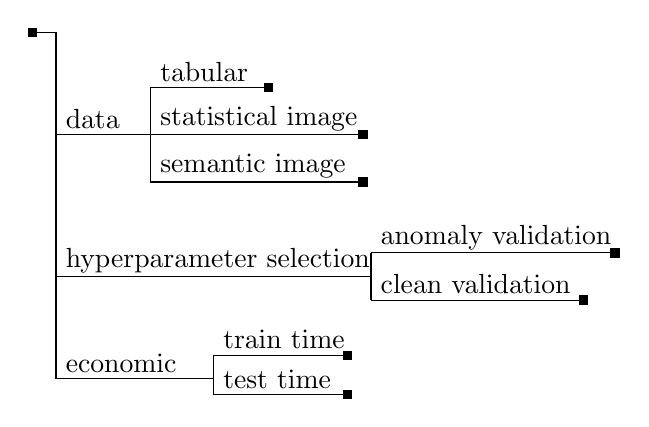
\begin{tikzpicture}
          \draw (-0.3,1.3) -- (0,1.3);
          \draw (0,1.3) -- (0,-3.1);
          
          \filldraw ([xshift=-1.5pt,yshift=-1.5pt]-0.3,1.3) rectangle ++(3pt,3pt);

          \draw (0,0) -- (1.2,0);
          \node[anchor=west] at (0,0.2) {data};
          \draw (1.2,-0.6) -- (1.2,0.6);
          \node[anchor=west] at (1.2,0.8) {tabular};
          \filldraw ([xshift=-1.5pt,yshift=-1.5pt]2.7,0.6) rectangle ++(3pt,3pt);
          \draw (1.2,0.6) -- (2.7,0.6);
          \node[anchor=west] at (1.2,0.2) {statistical image};
          \filldraw ([xshift=-1.5pt,yshift=-1.5pt]3.9,0) rectangle ++(3pt,3pt);
          \draw (1.2,0) -- (3.9,0);
          \node[anchor=west] at (1.2,-0.4) {semantic image};
          \filldraw ([xshift=-1.5pt,yshift=-1.5pt]3.9,-0.6) rectangle ++(3pt,3pt);
          \draw (1.2,-0.6) -- (3.9,-0.6);
          
          \draw (0,-1.8) -- (4,-1.8);
          \node[anchor=west] at (0,-1.6) {hyperparameter selection};
          \draw (4,-1.5) -- (4,-2.1);
          \filldraw ([xshift=-1.5pt,yshift=-1.5pt]7.1,-1.5) rectangle ++(3pt,3pt);
          \draw (4,-1.5) -- (7.1,-1.5);
          \node[anchor=west] at (4.0,-1.3) {anomaly validation};
          \filldraw ([xshift=-1.5pt,yshift=-1.5pt]6.7,-2.1) rectangle ++(3pt,3pt);
          \draw (4,-2.1) -- (6.7,-2.1);
          \node[anchor=west] at (4.0,-1.9) {clean validation};
          
          \draw (0,-3.1) -- (2,-3.1);
          \node[anchor=west] at (0,-2.9) {economic};
          \draw (2,-2.8) -- (2,-3.3);
          \filldraw ([xshift=-1.5pt,yshift=-1.5pt]3.7,-2.8) rectangle ++(3pt,3pt);
          \draw (2,-2.8) -- (3.7,-2.8);
          \node[anchor=west] at (2,-2.6) {train time};
          \filldraw ([xshift=-1.5pt,yshift=-1.5pt]3.7,-3.3) rectangle ++(3pt,3pt);
          \draw (2,-3.3) -- (3.7,-3.3);
          \node[anchor=west] at (2,-3.1) {test time};
          

    \end{tikzpicture}
    
    \caption{Various aspects of anomaly detection comparison forming the \textit{context} of the experiment.}
    \label{fig:context}
\end{figure}

While many practitioners are eager to see which method is the best for their application, the specifics of the application may differ. We have conducted a large number of experiments to identify the main sources of variability influencing the performance of anomaly detection methods. The number of combinations of these aspects is huge. Therefore, we identified the key axes of variability: datasets, hyperparameter selection strategy, and economic point of view. From these axes, we select a few discrete points, on which we will provide a comparison. The particular combination of the selected aspect will be called \emph{context}, see Fig.~\ref{fig:context} for illustration. 

The first axis is the target data domain. Our experiments used two types of datasets: \textit{tabular} and \textit{image}. This is the most obvious split, and indeed most authors of prior art test their methods on either choice of data. Another possible way to look at data is whether they contain \textit{statistical} or \textit{semantic} anomalies. Statistical anomalies should be located in areas of a low likelihood of the normal class, while semantic~\cite{ahmed2020detecting} anomalies cannot be differentiated from normal data statistically. This is because they appear in datasets with multiple sources of variations, where only some of them are considered anomalous. Such types of anomalies are most common in image datasets.  Imagine a detector that aims to learn a representation of birds from images without preprocessing. Most of the bird pictures are going to have the sky in the background. Since the background occupies most of a picture and therefore has a strong signal, a bird on grass is going to be a statistical anomaly, while an airplane with sky in the background is an example of a semantic anomaly in case the original goal was to identify pictures that do not contain a bird. The suitability of the tested methods for the dataset context axis is studied in Sec.~\ref{sec:dataset_context}.

The second axis of variability is the hyperparameter selection strategy. It should be a gold standard that the experiments are repeated on different splits of data to training, validation, and testing subsets, especially if the datasets are small. However, in most of the reviewed recent papers~\cite{liu2019generative,wang2020advae,schlegl2017unsupervised, akcay2018ganomaly, perera2019ocgan}, this procedure was not mentioned with the exception of~\cite{ruff2018deep}. Therefore, our comparison fills this gap. Also, it is important to define the nature of information available for the selection of the hyperparameters: it is indeed a very different task if there is some (often small) number of known anomalies in the validation dataset that can be used to choose hyperparameters by cross-validation or if the validation dataset is clean. In our experience, the former case is more common. Our observations are summarised in Sec.~\ref{sec:hyperparameter_context}.

The third axis is the economic aspect of a problem. There might be serious computational restrictions present in solving real-life problems. One might then not opt for a method that promises state-of-the-art performance, but for another that reaches slightly worse performance but can be trained economically, and its performance is robust with regards to hyperparameter optimization. More details on this can be found in Sec.~\ref{sec:economic_context}.

Finally, Sec.~\ref{sec:other_context} contains other influences that we have originally considered to be important but eventually did not prove to make a significant difference in comparison of multiple methods. These include the use of performance measures other than traditional AUC, the use of Bayesian optimization, and others. 

\section{Compared methods}
\label{sec:comparedmethods}
This section briefly reviews deep generative models in the order of exactness of calculation of likelihood. Therefore, it starts with flow models, continues with probabilistic (variational) autoencoders, where the prior art on the application in anomaly detection is rich, and finishes with generative adversarial networks where the calculation of any score related to likelihood is dubious at best. We specifically focus on issues that affect the performance of the method for anomaly detection, most often the anomaly score, if it is not rigorously defined. We also briefly review other examples of deep methods that are relevant for the comparison, such as two-stage models and distance-based models that are not generative but can be used in anomaly detection. We do not review classical methods here, as this has been done many times elsewhere, but we list them in the relevant experimental section.

Before the description, we introduce a notation. Training samples, $\vec{x},$ are assumed to be i.i.d from the underlying probability distribution $p({\vec{x}})$ defined on the input space $\mathcal{X}$. Following the conventional definition of an anomaly~\cite{barnett1974outliers}, each anomaly detection method is expected to provide a quantity (called score and denoted $s(\vec{x}')$) related to the probability of a sample $\vec{x}'$ being generated from $p(\vec{x}).$ The score does not need to be a normalized distribution, as the threshold is typically determined as an empirical estimate of the quantile. Most functions in this section are assumed to have parameters optimized during training. 

\subsection{Normalizing flows}
The name normalizing flows refers to methods relying on the change of variables formula
\begin{equation}
    p\left(\vec{x}\right) = p\left(\vec{z}\right)\!\left\vert \text{det} J_f\!\left(\vec{z}\right) \right\vert^{-1}, \, \vec{z} = f^{-1}\!\left(\vec{x}\right),
\label{eq:rv_transformation}
\end{equation}
where $J_f\!\left(\vec{z}\right)$ is Jacobi matrix of function $f$ evaluated at $\vec{z}$. $p(\vec{z})$ is a known distribution of the latent variable $\vec{z}$ from space $\mathcal{Z}$ of the same dimension as $\mathcal{X}$.

Theoretical reviews~\cite{papamakariosNormalizingFlowsProbabilistic2019, kobyzevNormalizingFlowsIntroduction2020} require $f$ to be invertible and both $f$ and $f^{-1}$ to be differentiable. Therefore, flow models primarily differ in how they define the class of functions $f$, which ranges from simple affine transformations to solutions of ordinary differential equations. The expressive power comes from their composition, as is usual in neural networks. In the comparison, we consider flows on tabular data only, for which we have implemented the well-known RealNVP~\cite{dinh2016density} and MAF~\cite{papamakariosMaskedAutoregressiveFlow2018} flows alongside a promising class of Sum-Product-Transform networks --- SPTN~\cite{pevny2020sum} combining normalizing flows with a graphical model. The likelihood is used as a natural anomaly score.

Flow models have not yet enjoyed much popularity in anomaly detection~\cite{yamaguchi2019adaflow, schmidtNormalizingFlowsNovelty2019, diasAnomalyDetectionTrajectory2020a, pevny2020sum} in comparison to the autoencoder-based models reviewed below. To us, this is surprising since these methods can exactly calculate likelihood functions, which under a good fit are the ideal anomaly score. Meanwhile, the focus of the surrounding community is on the topic of \textit{out of distribution detection} (OOD)\footnote{Out of distribution detection means identifying samples coming from a different dataset. For example, a model trained on MNIST / CIFAR10 should assign a low likelihood to samples from Fashion MNIST / SVHN respectively.}~\cite{nalisnickDeepGenerativeModels2019}, which is very related to anomaly detection if not being equal. Ref.~\cite{choiWAICWhyGenerative2019} suggests to use ensembles, while~\cite{renLikelihoodRatiosOutofDistribution2019} recommends to convert the single-class problem to classification problems in the spirit of \cite{steinwart2005a}. A deep investigation of OOD in~\cite{kirichenkoWhyNormalizingFlows2020} shows that with low-level features such as pixel intensities, flows tend to learn local models, i.e. according to taxonomy in~\cite{ruff2020unifying} they fail to detect semantic anomalies.

\subsection{Autoencoder-based models}
\label{sec:ae_theory}
Autoencoder-based models differ from flows by relaxing the exact mapping between $\vec{x}=f(\vec{z})$ \eqref{eq:rv_transformation} into a probability distribution $p_{\vec{\theta}} (\vec{x}|\vec{z})=\mathcal{N}(\vec{\mu}_{\vec{\theta}}(\vec{z}), \mathrm{diag}(\vec{\sigma}_{\vec{\theta}}(\vec{z})))$,\footnote{Other forms of the distribution are possible, e.g. Bernoulli for scaled pixel intensities.} called \emph{decoder}. The symbol $\vec{\theta}$ denotes the trainable parameters of the decoder, e.g. weights of a neural network. The marginal likelihood is computed as
\begin{equation}
    p(\vec{x})=\int p_{\vec{\theta}}(\vec{x}|\vec{z})p(\vec{z}) d\vec{z},
    \label{eq:vae-px}
\end{equation}
where $p(\vec{z})$  is a chosen prior probability distribution of the latent variable. This relaxation allows for more flexible models, e.g. using different dimension of $\vec{x}$ and $\vec{z}$. However, training and evaluation of the model is more demanding since the marginal likelihood \eqref{eq:vae-px} is not available in closed form. Therefore~\cite{kingma2013auto} introduces \emph{encoder} distribution $q_{\vec{\phi}}(\vec{z}|\vec{x})=\mathcal{N}(\vec{\mu}_{\vec{\phi}}(\vec{x}), \mathrm{diag}(\vec{\sigma}_{\vec{\phi}}(\vec{x})))$  with parameters $\vec{\phi}$ allowing approximation of Eq.~\eqref{eq:vae-px} as described below in Eq.~\ref{eq:vae_loss}.

Various modifications of the original formulation have been proposed, giving rise to many specialized methods. Below we describe extensions in three blocks according to i) approximation of the likelihood \eqref{eq:vae-px} used for training, ii) prior model, iii) approximations used for evaluating the anomaly score, and iv) various modifications of the original concept.

\paragraph{Training loss}
The original Variational Autoencoder~\cite{kingma2013auto} (VAE) proposes to replace \eqref{eq:vae-px} by the evidence lower bound (ELBO)
\begin{equation}
    \mathcal{L}_{\text{VAE}} (\vec{\theta}, \vec{\phi}) = - \mathbb{E}_{q_{\vec{\phi}}(\vec{z}|\vec{x})} \left[ \log p_{\vec{\theta}}(\vec{x}|\vec{z}) \right] + D_{KL} \left( q_{\vec{\phi}}(\vec{z}|\vec{x}) || p(\vec{z}) \right),
\label{eq:vae_loss}
\end{equation}
which combines reconstruction error with regularization term is form of the Kullback-Leibler divergence (KLD) between the encoder distribution and the prior. Models based on~\eqref{eq:vae_loss} will be referred to as the VAE family.

Asymmetry of the KL divergence motivated search for a more accurate metric. Ref.~\cite{tolstikhin2017wasserstein} proposes to replace KL by a Wasserstein divergence, yielding training loss function in the form:
\begin{equation}
    \mathcal{L}_{\text{WAE}} (\vec{\theta}, \vec{\phi}) = - \mathbb{E}_{q_{\vec{\phi}}} \left[ \log p_{\vec{\theta}}(\vec{x}|\vec{z}) \right] + \lambda D \left( q_{\vec{\phi}}(\vec{z}|\vec{x}) || p(\vec{z}) \right),
\label{eq:wae_loss}
\end{equation}
where $\lambda >0$  is a scalar hyperparameter, and $D$  is an arbitrary divergence. The most commonly used divergence is the kernelized maximum-mean-discrepancy (MMD) with kernel  $k$, which was reported to perform well in matching high dimensional distributions~\cite{zhao2017infovae}. Models based on~\eqref{eq:wae_loss} will be referred to as the WAE  family.

An alternative choice of the divergence $D$ in~\eqref{eq:wae_loss} proposed in~\cite{tolstikhin2017wasserstein} is the adversarial loss, which in combination with the Gaussian decoder coincides with the adversarial autoencoder~\cite{makhzani2015adversarial}. This divergence introduces a third network $d_{\vec{\psi}}(\vec{z}):\mathcal{Z} \rightarrow \left[ 0,1 \right]$,  called discriminator, trained to distinguish between samples from the prior $p(\vec{z})$ and samples $x$ projected by the encoder $q(z|x)$. Every step of optimization separately updates the autoencoder and discriminator parts to minimize the loss functions
\begin{align}
\label{eq:aae_loss}
\mathcal{L}_{\text{AE}}(\vec{\theta}, \vec{\phi}) & = - \mathbb{E}_{q_{\vec{\phi}}(\vec{z}|\vec{x})} \left[ \log p_{\vec{\theta}}(\vec{x}|\vec{z}) \right] - \lambda \log d_{\vec{\psi}}(\vec{z}^q), \\
\mathcal{L}_{\text{D}}(\vec{\psi}) & = \log d_{\vec{\psi}}(\vec{z}^p) + \log \left(1-d_{\vec{\psi}}(\vec{z}^q)\right),
\end{align}
respectively, where $\vec{z}^p \sim p(\vec{z})$, $\vec{z}^q \sim q_{\vec{\phi}}(\vec{z}|\vec{x})$. Models trained with loss function~(\ref{eq:aae_loss}) will be denoted as AAE.

\paragraph{Prior model}
A common criticism of the VAE model is its use of the standard Gaussian prior $p(z),$ which stimulates the distribution $q(z|x)p(x)$ to have a single mode, and therefore it is hard to fit data with a multi-modal latent distribution. Ref.~\cite{tomczak2018vae} proposes a learnable multimodal \emph{Vamp} prior realized as a mixture of $K$ independent Gaussian components. Vamp prior is compatible with AAE and WAE models since it does not have an analytical expression of KLD in~\eqref{eq:vae_loss}. The mean values of components of the mixture are learned together with the parameters of the autoencoder. In the model selection below, the Vamp prior is considered as a binary hyperparameter with an additional parameter, $K,$ specifying the number of components.

\paragraph{Anomaly Score}
The likelihood function \eqref{eq:vae-px} also constitutes the ideal anomaly score. Some training losses such as ELBO \eqref{eq:vae_loss} were designed as approximations of the likelihood and can thus be used as anomaly scores. However, this interpretation is not so clear for other  training losses, i.e. \eqref{eq:wae_loss}, \eqref{eq:aae_loss}, hence their authors propose anomaly scores as part of the method. Nevertheless, many scores are interchangeable, giving rise to another degree of freedom (hyperparameter) for the use of autoencoders in anomaly detection. A common score is based on the first term in the loss i.e. a Monte Carlo estimate of the expectation of conditional log-likelihood over the encoder, yielding \begin{align}
s_{\text{rs}}(\vec{x}) = & - \frac{1}{L}\sum_{l=1}^L \log p_{\vec{\theta}}(\vec{x}| \vec{z_l}),   \vec{z}_l \sim q_{\vec{\phi}}(\vec{z}|\vec{x}). \label{eq:score_sample}
\end{align}
This score, called sampled reconstruction error (abbreviated as rs), was shown in~\cite{xu2018unsupervised} to be more accurate than evaluating~\eqref{eq:vae-px} by sampling $z$ from the prior $p(\vec{z})$. Further simplification is based on replacing samples from the encoder  by its mean, yielding the common reconstruction error score (abbreviated as rm)
\begin{align}
s_{\text{rm}}(\vec{x}) = & - \log p_{\vec{\theta}}(\vec{x}| \vec{\mu}_{\vec{\phi}}(\vec{x})) \label{eq:score_mean}
\end{align}
The usage of~\eqref{eq:score_mean} is justified by the assumption that taking the mean at the encoder should approximate~\eqref{eq:score_sample} while having lower computational demands. For adversarial autoencoders, these simplifications can be combined with the discriminator score~\cite{schlegl2017unsupervised, zenatiEfficientGANBasedAnomaly2018},
\begin{equation}
    s_{\text{a}}(\vec{x}) = \alpha s_{\text{rm}}(\vec{x}) + (1-\alpha) d_{\vec{\psi}}(\vec{\mu}_{\vec{\phi}}(\vec{x})), \alpha \in \left[ 0, 1 \right].
\label{eq:aae_score}
\end{equation}

The reconstruction error-based anomaly scores were criticized in~\cite{pidhorskyi2018generative}  for not capturing the true data density $p(\vec{x}).$ The proposed replacement is based on the orthogonal decomposition of the data into $x=x^\bot +x^{\parallel} $ where the $x^\parallel$  lies in the tangent space of to the manifold defined by the decoder. This allows to decompose the marginal likelihood into a product of two orthogonal parts
\begin{equation}
    p(\vec{x}) \approx p(\vec{x}^{||})p(\vec{x}^{\perp}),
\label{eq:jacodeco}
\end{equation}
where $p(\vec{x}^\bot)$ is the reconstruction error, and $p(\vec{x}^\parallel)$ is obtained by transformation of variables~\eqref{eq:rv_transformation}. This score is abbreviated as \textit{jc} in the following text. The calculation of~\eqref{eq:jacodeco} is expensive, as it needs to compute the singular value decomposition of the Jacobian. For implementation details, see~\cite{pidhorskyi2018generative} or~\cite{vsmidl2019anomaly}.

\paragraph{Other models and techniques}
 A plethora of models based on probabilistic autoencoders and specialized for anomaly detection was introduced in recent years, such as~\cite{zong2018deep, pereira2018unsupervised, xu2018unsupervised, principi2017acoustic, chen2018unsupervised, chalapathyGroupAnomalyDetection2018}. Below, we list models included in the comparison and not described above.

The self-adversarial Variational Autoencoder (adVAE)~\cite{wang2020advae} was included because it claims superiority over the state-of-the-art methods, such as VAE, DAGMM~\cite{zong2018deep}, WGAN-GP~\cite{gulrajani2017improved} or MO-GAAL~\cite{liu2019generative} on tabular datasets. It augments the usual encoder-decoder pair with a transformer, whose goal is to simulate anomalies during training. The seeming flaw of the model is that it is trained only on normal data, and there is no link between the real and the simulated anomalies. The sampled reconstruction is used as an anomaly score.

Despite its name, GANomaly~\cite{akcay2018ganomaly, ahnDeepGenerativeModelsBased2020} is more related to adversarial autoencoders than to GANs. It consists of encoder-decoder-encoder architecture with a discriminator, similar to an AAE. The anomaly score is the difference between latent representations of a sample after the first and second encoding. An upgrade to this model, skip-GANomaly~\cite{akcay2019skip}, uses skip connections in a U-Net type architecture. Here, the anomaly score is a combination of reconstruction error and feature-matching loss (see the next section on fmGAN). Although originally proposed only for use in images, we have implemented a variant for tabular data as well.  

\subsection{Generative adversarial networks} \label{sec:gan}
Generative adversarial networks~\cite{goodfellow2014generative} construct and train two networks: a generator $g_{\vec{\phi}}(\vec{z}):\mathcal{Z} \rightarrow \mathcal{X}$ and a discriminator $d_{\vec{\psi}}(\vec{x}) :\mathcal{X} \rightarrow \left[ 0,1 \right]$ approximating the probability
of $\vec{x}$ being a sample from the data distribution rather than the generator. The generator aims to transforms samples from $p(\vec{z}) = \mathcal{N}(\vec{0}, \vec{I})$ to $\mathcal{X}$ such that they are indistinguishable from the real data. Formally, the  optimization objectives are
\begin{align}
\mathcal{L}_{\text{d}}(\vec{\psi}) = & \log d_{\vec{\psi}}(\vec{x}) + \log \left( 1 - d_{\vec{\psi}}(g_{\vec{\phi}}(\vec{z})) \right) , \\
    \mathcal{L}_{\text{g}}(\vec{\phi}) = &- \log d_{\vec{\psi}}(g_{\vec{\phi}}(\vec{z})),\label{eq:gan-Lg}
\end{align}
where $\mathcal{L}_d$ is maximized while $\mathcal{L}_g$  is minimized, $\vec{z}$ is sampled from the prior and $\vec{x}$ from the training set. The optimization searches the saddle point of the two losses, which is difficult and notoriously unstable. Therefore a long series of work, e.g.~\cite{hong2019generative}, proposes improvements over the basic approach~\cite{goodfellow2014generative}. One of the approaches is based on the introduction of  feature-matching loss~\cite{salimans2016improved}. We will denote the model trained with this loss as feature-matching GAN  (fmGAN). In fmGAN training, the cost function of the generator~\ref{eq:gan-Lg} is augmented with output of some intermediate layer of the discriminator. Specifically, the generator is optimized as 
\begin{equation}
    \mathcal{L}_{\text{fm}}(\vec{\phi}) = \alpha \mathcal{L}_{\text{g}}(\vec{\phi}) + || h_{\vec{\psi}}(\vec{x}) - h_{\vec{\psi}}(g_{\vec{\phi}}(\vec{z})) ||^2,
    \label{eq:fmloss}
\end{equation}
where $h_{\vec{\psi}}$ is the output of the intermediate layer of the discriminator and $\vec{z}$ is a sample from $p(\vec{z})$. This feature-matching loss is used in AnoGAN~\cite{schlegl2017unsupervised} for detection of anomalous objects in images, with hyperparameter $\alpha$, which was zero in the original publication \cite{salimans2016improved}. 

GANs are frequently augmented with a third model $q(z|x)$~\cite{donahue2016adversarial} which makes the distinction between GANs and VAEs blurred, as demonstrated by using min-max (GAN-like) approximation of Wasserstein divergence in Wasserstein autoencoders, Sec.~\ref{sec:ae_theory}.  This makes it sometimes hard to assign a model to some class (for example, GANomaly belongs to probabilistic autoencoders in our opinion).

Recall the role of the discriminator is to discriminate \textit{generated} samples from \textit{real} ones. Since the generator is trained to generate samples with a high discriminator score, it seems logical to use the discriminator to score anomalies
\begin{equation}
     s_{\text{GAN}}(\vec{x}) = 1 - d_{\vec{\psi}}(\vec{x}),
     \label{eq:disc_score}
\end{equation}
which is used e.g., in~\cite{liu2019generative}. The common critique is that the discriminator was not trained to recognize an arbitrary distribution of the anomalies but only that of the latent transformed by the generator. Thus it may fail to recognize anomalous samples of interest. 

AnoGAN recognizes this flaw and proposes to augment the discriminator loss~\eqref{eq:fmloss} for training and an iterative procedure that searches for the latent code $z$ most likely to generate the tested sample to identify anomalous images. However, this procedure is computationally expensive. Its sequel, f(ast)AnoGAN~\cite{schleglFAnoGANFastUnsupervised2019}, uses Wasserstein GAN with gradient penalization~\cite{gulrajani2017improved} to improve stability and adds $q(z|x)$ to find $z$ closest to given $x$ in $q(x|z)$ faster. The anomaly score of fAnoGAN is a combination of discriminator score and feature-matching loss.

Multiple-Objective Generative Adversarial Active Learning (MOGAAL)~\cite{liu2019generative}, train $k$ generators against a single discriminator on input data divided into $k$ subsets. The usual discriminator score in Eq.~\eqref{eq:disc_score} is used to test new samples.
Other anomaly detection models derived from GAN include~\cite{zenatiEfficientGANBasedAnomaly2018, kliger2018novelty, perera2019ocgan}, however, it seems that autoencoder-based models are more popular for anomaly detection, and our selected candidates are representative.

\subsection{Two-stage models}
A recurring idea~\cite{ergen2017unsupervised, yaoUnsupervisedAnomalyDetection2019, ruff2018deep, vskvara2020detection} is to combine autoencoders with a secondary model acting on the latent space defined by the encoder. The motivation behind it is that the encoder should preserve the semantic information of the sample and remove noise (e.g. background in images). Additionally, reducing the size mitigates the curse of dimensionality, as high dimensions can be problematic for some models.

We are not aware of a general term for this approach. We use the term \textit{two-stage models}, following~\cite{dai2019diagnosing}, although~\cite{chalapathy2019deep} uses the term \textit{deep hybrid models}. In~\cite{ruff2018deep}, the model optimizes the projection of data (by virtue of NNs) to a new space, where they can be easily enclosed in a sphere of minimum radius. The approach presented in~\cite{vskvara2020detection, yaoUnsupervisedAnomalyDetection2019} explicitly splits the creation of the detector into two parts. It first trains a VAE (and its variants), and then it fixes the encoder. The anomaly score is calculated by a kNN \cite{vskvara2020detection} or by OC-SVM \cite{yaoUnsupervisedAnomalyDetection2019} detectors in the latent space, obtained by projecting the sample by the fixed encoder. The two-stage models can also be viewed as a kNN with a trained metric or OC-SVM with a trained kernel. The embedding can be optimized differently, for example, by enforcing the margin between anomaly candidates and normal data as done in the REPEN~\cite{pangLearningRepresentationsUltrahighdimensional2018} method, which uses an ensemble of 1NN detectors as the second stage.

\section{Experimental setup}
\label{sec:experimentalsetup}
\subsection{Datasets}
\label{sec:datasets}
Two criteria guided the choice of datasets (mainly the tabular ones): first, they ought to be publicly available, and second, they should appear in surveys or articles presenting new methods.  In total, we have collected $40$ tabular datasets, the majority of which came from the UCI repository~\cite{Dua:2019}. Except for ANNThyroid, Arrhytmia, HAR, HTRU2, KDD Cup 99 (small), Spambase, Mammography, and Seismic, where the anomaly class has a clear meaning (security incident or disease), we have followed the technique of~\cite{emmott2013systematic} for creating artificial datasets for anomaly detection tasks from classification datasets. More precisely, we have used only "easy" and "medium" anomalies, as "hard" and "very hard" are not truly anomalous in the sense of being statistically distinct from the normal class. Prior to model training, features on tabular datasets were normalized to have zero mean and unit variance. Further details of the datasets are provided in Tab.~\ref{tab:tabular_datasets}.

The number of image datasets used for the evaluation of deep models is limited, as there are very few datasets designed purely for anomaly detection - MNIST-C~\cite{muMNISTCRobustnessBenchmark2019} and MVTec-AD~\cite{bergmannMVTecADComprehensive2019}. Therefore, we have decided to extend these with artificially created anomaly datasets based on common image datasets MNIST~\cite{lecun-mnisthandwrittendigit-2010}, FashionMNIST~\cite{xiao2017fashion}, CIFAR10~\cite{krizhevsky2009learning}, and SVHN2~\cite{netzer2011reading}. These are also used for anomaly detection tasks in the prior art~\cite{perera2019ocgan, pidhorskyi2018generative, ruff2018deep}. A single class (of digits/objects) is often considered normal and the rest anomalous, which is the primary setting of our experiments. Only three subsets \textit{wood, grid, transistor} of the MVTec-AD dataset were used due to our computational constraints. These were chosen since they represent problems of various degrees of difficulty. Downsampling to $128 \times 128$ was required to fit the computational envelope for most methods on the real-world high-resolution images in MVTec-AD.  We have linearly extrapolated the image data when training GANomaly so that the input dimensions were a multiple of 16 (this is a result of the model's fixed architecture). No other preprocessing has been applied prior to training since the source data already have all channels scaled to [0,1].  Basic statistics on image datasets are shown in table Tab.~\ref{tab:image_datasets}. 

We have performed a visual inspection of the nature of anomalies in the image datasets; see Supplementary~\ref{sec:appendix_extending_image_results}. Since most of the manually processed datasets (MNIST, FashionMNIST, MVTec-AD, and MNISTC) have a rich and consistent number of samples in the normal class and clear anomalies, we consider them to be statistical anomalies. On the other hand, images in the majority of classes in CIFAR10 and SVHN2 have a strong background and are thus considered to contain semantic anomalies. This prior division is also supported by a different behavior of different methods as reported in the Supplementary, Fig.~\ref{fig:image_knowledge_rank_pat_auc}. 

\subsection{Data splits and experiment repetitions}
\label{sec:repetitions}
The experiments on tabular data and MNIST-C/MVTec-AD image datasets were repeated five times with different random cross-validation splits. Specifically, in each repetition (five in total) of an experiment with the same model hyperparameters, the \textit{normal data} in each dataset was randomly split in 60\%/20\%/20\% ratios to train/validation/test subsets, respectively. \textit{Anomalous data} were split such that 50\% were in the validation part and 50\% in the testing part, which means the training subset has not contained anomalous samples. \footnote{A training set without any anomalies is in practice very optimistic, but this decision removes another degree of freedom from the evaluation for the sake of clarity of results.} The proportion of anomalies that were used in the validation phase varied from zero to the selected 50\%. 

Due to the already substantial computational requirements on the rest of the image datasets, we have not trained models with the same hyperparameters on repeated random cross-validation splits. In our experience, the results on different splits of these datasets are almost the same since the number of samples is large and our trial experiments (see Supplementary Tab.~\ref{tab:images_seed_consistency}) have not exhibited a significant variation between the different random cross-validation experiment repetitions. 

\begin{table}
\centering
\tabcolsep=0.1cm
\begin{tabular}{llrrr}
\toprule
\textbf{dataset} & \textbf{alias} & \textbf{dim} & \textbf{anom} & \textbf{normal}   \\\midrule
ANNthyroid & ann  & 21 & 534 & 6665 \\
Arrhythmia & arr  & 275 & 206 & 245 \\
HAR & har & 561 & 1944 & 8355  \\
HTRU2 & htr & 8 & 1638 & 16257  \\
KDD99 (10\%) & kdd & 118 & 396742 & 97276  \\
Mammography & mam & 6 & 260 & 10921  \\
Seismic & sei  & 24 & 170 & 2412  \\
Spambase & spm & 57 & 1812 & 2786  \\
\midrule
Abalone & aba & 10 & 50 & 2151  \\
Blood Transfusion & blt & 4 & 16 & 382  \\
Breast Cancer Wisconsin & bcw  & 30 & 206 & 356 \\
Breast Tissue & bts & 9 & 22 & 65 \\
Cardiotocography & crd & 27 & 228 & 1830  \\
Ecoli & eco & 7 & 108 & 205  \\
Glass & gls & 10 & 94 & 112  \\
Haberman & hab & 3 & 14 & 225  \\
Ionosphere & ion & 33 & 122 & 225  \\
Iris & irs & 4 & 46 & 100  \\
Isolet & iso & 617 & 3300 & 4496  \\
Letter Recognition & ltr & 617 & 3600 & 4196  \\
Libras & lbr & 90 & 142 & 215  \\
Magic Telescope & mgc & 10 & 3882 & 12331  \\
Miniboone & mnb & 50 & 23922 & 93565  \\
Multiple Features & mlt & 649 & 800 & 1200  \\
PageBlocks & pgb & 10 & 384 & 4911  \\
Parkinsons & prk & 22 & 44 & 146  \\
Pendigits & pen & 16 & 5384 & 5537  \\
Pima Indians & pim & 8 & 176 & 500  \\
Sonar & snr & 60 & 96 & 110  \\
Spect Heart & sph & 44 & 52 & 211  \\
Statlog Satimage & sat & 36 & 2630 & 3592  \\
Statlog Segment & seg & 18 & 938 & 1320  \\
Statlog Shuttle & sht & 8 & 28 & 57767  \\
Statlog Vehicle & vhc & 18 & 132 & 627  \\
Synthetic Control Chart & scc & 60 & 200 & 400  \\
Wall Following Robot & wrb & 24 & 2220 & 2921  \\
Waveform-1 & wf1 & 21 & 1482 & 3302  \\
Waveform-2 & wf2 & 21 & 1472 & 3302  \\
Wine & wne & 13 & 70 & 106  \\
Yeast & yst & 8 & 390 & 751   \\\bottomrule
\end{tabular}
\vspace*{0.15cm}
\caption{Basic statistics of the tabular dataset designed for anomaly detection  (above split) and multi-class datasets  (bellow split).}
\label{tab:tabular_datasets}
\end{table}

\begin{table}
    \centering
    \tabcolsep=0.1cm
    \begin{tabular}{lllrr}
    \toprule
    \textbf{dataset} & \textbf{alias} & \textbf{dim} & \textbf{anom} & \textbf{normal} \\
    \midrule
    MNIST-C & mnistc & 28x28x1 & 70000 & 70000 \\
    MVTec-AD - wood & wood & 1024x1024x3 & 60 & 266 \\
    MVTec-AD - grid & grid & 1024x1024x3 & 57 & 285 \\
    MVTec-AD - transistor & transistor & 1024x1024x3 & 40 & 273 \\
    \midrule
    CIFAR10 & cifar10 & 32x32x3 & 54000 & 6000  \\
    FashionMNIST & fmnist & 28x28x1 & 63000 & 7000   \\
    MNIST & mnist & 28x28x1 & 63686 & 6312  \\
    SVHN2 & svhn2 & 32x32x3 & 80327 & 18960  \\\bottomrule
    \end{tabular}
    \vspace*{0.15cm}
    \caption{Basic statistics of image datasets designed for anomaly detection (above split) and multi-class datasets (below split).}
    \label{tab:image_datasets}
\end{table}

\subsection{Notes on implementation of models}
As mentioned in the introduction, we have compared various types of \textit{deep} methods to \emph{classical} ones serving as an etalon. Classical methods included ABOD~\cite{kriegel2008angle}, HBOS~\cite{goldstein2012histogram}, LODA~\cite{pevny2016loda}, LOF~\cite{breunig2000lof}, IsolationForest~\cite{liu2008isolation}, OC-SVM~\cite{scholkopf2001estimating}, PIDForest~\cite{gopalanPIDForestAnomalyDetection2019}, and kNN~\cite{ramaswamy2000efficient}. For ABOD, HBOS, and LODA, we have used pyOD library~\cite{zhao2019pyod} implementation, for LOF, IsolationForest, and OC-SVM we used scikit-learn~\cite{scikit-learn} implementation, and last but not least we have used our own implementation of kNN. The acronyms used in the result section are summarized in Tab.~\ref{tab:model_acronyms_2col} together with the classification of the deep methods as described in Sec.~\ref{sec:comparedmethods}.

Since image datasets are typically much larger than tabular, the OC-SVM was implemented as an ensemble of 10 OC-SVM models trained disjoint subsets of data, see Sec.~\ref{sec:appendix_implementation}, because it has at best $O(n^2)$ scaling in the number of samples. 

To ensure consistency among deep models, we implemented all methods except the MOGAAL\footnote{The pyOD implementation was used.} ourselves using the Flux~\cite{innes:2018} framework in Julia~\cite{Julia-2017} language. Apart from the models mentioned in Sec.~\ref{sec:comparedmethods}, we have also implemented DeepSVDD~\cite{ruff2018deep}, DAGMM~\cite{zong2018deep} and REPEN~\cite{pangLearningRepresentationsUltrahighdimensional2018}, which have been included in multiple comparisons~\cite{ruff2020unifying, wang2020advae, chalapathy2018anomaly}.

\begin{table}
    \centering
    \tabcolsep=0.1cm
    
    \begin{tabular}{cll|cll}
    \toprule
    \textbf{class} & \textbf{model} & \textbf{acronym} & \textbf{class} & \textbf{model} & \textbf{acronym}  \\\midrule
    
    \parbox[t]{2mm}{\multirow{3}{*}{\rotatebox[origin=c]{90}{flows}}} & MAF & maf & \parbox[t]{2mm}{\multirow{5}{*}{\rotatebox[origin=c]{90}{two-stage}}} & DAGMM & dgmm \\
        & RealNVP & rnvp & & DeepSVDD & dsvd \\
        & SPTN & sptn & & REPEN & rpn  \\
        & & & & VAE-kNN & vaek \\

    \parbox[t]{2mm}{\multirow{5}{*}{\rotatebox[origin=c]{90}{autoencoders}}} 
        & AAE & aae & & VAE-OC-SVM & vaeo \\
        & adVAE & avae & & & \\

        & GANomaly & gano & \parbox[t]{2mm}{\multirow{8}{*}{\rotatebox[origin=c]{90}{classical}}} & ABOD & abod \\

        & skipGANomaly & skip & & HBOS & hbos \\
        & VAE & vae & & IsolationForest & if \\
        & WAE & wae & & kNN & knn \\
        & & & & LODA & loda \\
    \parbox[t]{2mm}{\multirow{3}{*}{\rotatebox[origin=c]{90}{gans}}}
        & fAnoGAN & fano & & LOF & lof \\ 
        & fmGAN & fmgn & & OC-SVM & osvm \\
        & GAN & gan & & PidForest & pidf \\
        & MOGAAL & mgal & \\
    
    \bottomrule
    \end{tabular}

    \vspace*{0.15cm}
    \caption{Overview of the main classes of compared methods and the acronyms used in the text.}
    \label{tab:model_acronyms_2col}
\end{table}

We emphasize that while implementing models, we have carefully compared our implementations to the reference where possible and (or) verified that our experimental results are similar to those provided in the corresponding publication.

Neural networks were trained with the ADAM~\cite{kingma2014adam} optimizer with early stopping measuring the continued decrease of loss on the validation dataset. All deep models trained on all image datasets used convolutional layers. More implementation details are in the Supplementary materials Sec.~\ref{sec:appendix_implementation}. The implementation code in the form of a Julia package can be found at \textbf{https://github.com/aicenter/GenerativeAD.jl}.

\subsection{Hyperparameters and their optimization}
\label{sub:hyperparameteroptimization}
Properly exploring the space of hyperparameters of all models is paramount to achieving fair and comparable experimental comparison, yet this is often superficially treated. Researchers often use \textit{default} or \textit{recommended} values ignoring that they are sub-optimal on datasets they use in their comparison. The conflicting results of the MOGAAL method in the original publication~\cite{liu2019generative} and in~\cite{wang2020advae} are a nice demonstration of this.  A prototypical example in the classical methods is OC-SVM, which is typically used with Gaussian kernel and with $\nu$ set to some default value, e.g. 0.05~\cite{pevny2016loda}, but can achieve better results with different kernels. The choice of hyperparameters in anomaly detection is everything but easy. But this means that the experimental settings should be set up such that all methods have been optimized equally. We conjecture that recommended and default values of hyperparameters are strongly correlated with the choice of evaluation datasets in the publications that recommend them.

\textit{Random grid search:} In order to explore the hyperparameter space of each method properly, we have employed a random search over a predefined grid for each method. This allows the construction of sections through the space for sensitivity studies. Moreover, it is frequently more efficient than grid search~\cite{bergstra2012random} and more flexible. For each model, dataset, and repetition, we have sampled 100 configurations from corresponding sets (see Tab.~\ref{tab:classical_hyperparameters}--\ref{tab:flow_hyperparameters}) and trained the models with them. In order to keep the neural-network-based models fixed across the repetitions on a single dataset, for each hyperparameter configuration we have also sampled a random seed that was used to initialize the network weights. To prevent running the training of expensive methods forever, there was a hard deadline of 24 hours in which the training of a single configuration for a given number of repetitions/classes should be finished. This automatically penalizes complicated models. 

Encoders for the two-stage models were selected from models performing best in terms of validation AUC or reconstruction error on the validation set. The second-stage models (kNN and OC-SVM) used hyperparameters sampled from Tab.~\ref{tab:classical_hyperparameters}. 

\textit{Bayesian optimization:} To overcome the limitation of random sampling in larger configuration spaces, we have also trained models whose hyperparameter choice was guided by Bayesian optimization of an evaluation metric on validation data. We followed the 50/50 strategy, where the underlying Gaussian process has been fitted with 50 randomly sampled configurations, and another 50 have been sampled based on the acquisition function. We have relied on the off-the-shelf implementation from the scikit-optimize framework~\cite{skopt} with default parameters.

\textit{Number of anomalies in the validation set:} A thorough exploration of the hyperparameter selection context also requires changing the criteria of model selection. When anomalies are available for validation, we select hyperparameters maximizing the AUC on the validation set. For experiments with no available anomalies, we have decided on the following hyperparameter selection mechanism. For \textit{classical} methods, we have used default hyperparameter values from literature - either authors of the method recommended them, they were used in a survey, or are default in a given implementation. Their overview is in Tab.~\ref{tab:default_hyperparameters}. For \textit{deep} methods, this is unfortunately impossible since their hyperparameter space is much larger, and the values are usually tuned to a specific dataset. Therefore, to have a universal solution, we have selected the already trained and evaluated models based on the lowest anomaly score on the normal validation data. This approach is theoretically justified for models with proper likelihood. 

\textit{Ensembles:} Some results on ensembles of anomaly detectors were already reported in~\cite{choiWAICWhyGenerative2019, nalisnickDeepGenerativeModels2019}. Since the other experiments required training a large number of models, it was decided to test whether even a naive approach to this problem brings some improvements. In order to mitigate some uncertainty given by different hyperparameter values, ensembles of detectors were constructed by averaging scores of some number of best-performing detectors. We have experimented with different fixed sizes of ensembles --- either top 10 or top 5. In such a case, the anomaly score is the average of the anomaly scores of ensemble members.

\textit{Performance criteria:} While the area under the ROC curve (AUC) is the most common criteria in anomaly detection, some authors use different metrics, such as partial AUC~\cite{dodd2003partial} or the true positive rate at a chosen false negative rate (TPR@). We have re-evaluated all results obtained for the random grid search on the TPR@5\%.

We have kept track of the time spent on the training of individual models and also on the time needed to evaluate them on validation and test sets. In total, we have trained 1,364,989 model instances in 9619 CPU days, evaluated 4,256,470 different scoring functions in 2704 CPU days, and created 10.2TB of experimental data.

\section{Experimental results}
\label{sec:results}
Before starting with the description of the experimental results, here we summarize conventions that are used unless said otherwise. The performance results are estimates of the AUC on the testing set and are averaged over five random cross-validation repetitions in the case of tabular and MvTec-AD/MNISTC image datasets. When ranks are reported, they are calculated by ordering methods on each dataset and calculating the average across them (as recommended in~\cite{demvsar2006statistical}). Hyperparameters are selected using the best average performance over 5 seeds or individually over 10 anomaly classes because the individual class splits constitute different anomaly detection problems. 

\begin{figure*}[h]
    \begin{tabular}{c c}
    \resizebox{\columnwidth}{!}{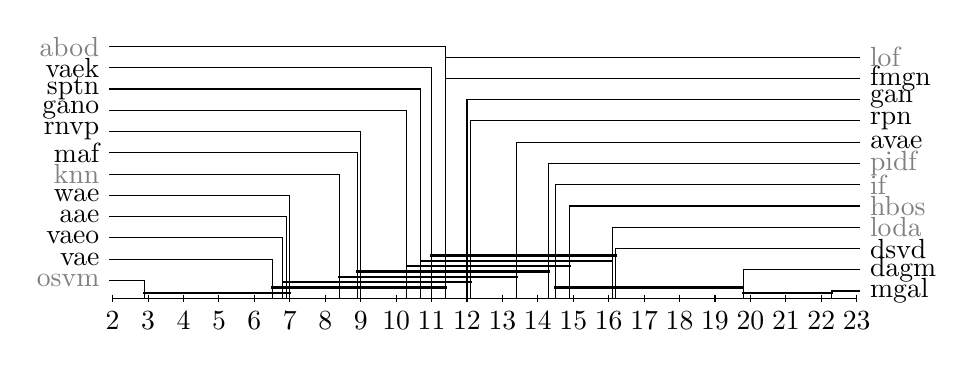
\begin{tikzpicture}[scale=0.45] 
  \draw (2.0,0) -- (23.0,0); 
  \foreach \x in {2,...,23} \draw (\x,0.10) -- (\x,-0.10) node[anchor=north]{$\x$}; 
  \draw (2.9,0) -- (2.9,0.5) -- (1.9, 0.5) node[anchor=east] {\textcolor{gray}{osvm}}; 
  \draw (6.5,0) -- (6.5,1.0999999999999999) -- (1.9, 1.0999999999999999) node[anchor=east] {vae}; 
  \draw (6.8,0) -- (6.8,1.6999999999999997) -- (1.9, 1.6999999999999997) node[anchor=east] {vaeo}; 
  \draw (6.9,0) -- (6.9,2.3) -- (1.9, 2.3) node[anchor=east] {aae}; 
  \draw (7.0,0) -- (7.0,2.9) -- (1.9, 2.9) node[anchor=east] {wae}; 
  \draw (8.4,0) -- (8.4,3.4999999999999996) -- (1.9, 3.4999999999999996) node[anchor=east] {\textcolor{gray}{knn}}; 
  \draw (8.9,0) -- (8.9,4.1000000000000005) -- (1.9, 4.1000000000000005) node[anchor=east] {maf}; 
  \draw (9.0,0) -- (9.0,4.7) -- (1.9, 4.7) node[anchor=east] {rnvp}; 
  \draw (10.3,0) -- (10.3,5.3) -- (1.9, 5.3) node[anchor=east] {gano}; 
  \draw (10.7,0) -- (10.7,5.9) -- (1.9, 5.9) node[anchor=east] {sptn}; 
  \draw (11.0,0) -- (11.0,6.5) -- (1.9, 6.5) node[anchor=east] {vaek}; 
  \draw (11.4,0) -- (11.4,7.1) -- (1.9, 7.1) node[anchor=east] {\textcolor{gray}{abod}}; 
  \draw (11.4,0) -- (11.4,6.8) -- (23.1, 6.8) node[anchor=west] {\textcolor{gray}{lof}}; 
  \draw (11.4,0) -- (11.4,6.2) -- (23.1, 6.2) node[anchor=west] {fmgn}; 
  \draw (12.0,0) -- (12.0,5.6) -- (23.1, 5.6) node[anchor=west] {gan}; 
  \draw (12.1,0) -- (12.1,5.0) -- (23.1, 5.0) node[anchor=west] {rpn}; 
  \draw (13.4,0) -- (13.4,4.4) -- (23.1, 4.4) node[anchor=west] {avae}; 
  \draw (14.3,0) -- (14.3,3.8) -- (23.1, 3.8) node[anchor=west] {\textcolor{gray}{pidf}}; 
  \draw (14.5,0) -- (14.5,3.2) -- (23.1, 3.2) node[anchor=west] {\textcolor{gray}{if}}; 
  \draw (14.9,0) -- (14.9,2.6) -- (23.1, 2.6) node[anchor=west] {\textcolor{gray}{hbos}}; 
  \draw (16.1,0) -- (16.1,1.9999999999999998) -- (23.1, 1.9999999999999998) node[anchor=west] {\textcolor{gray}{loda}}; 
  \draw (16.2,0) -- (16.2,1.4) -- (23.1, 1.4) node[anchor=west] {dsvd}; 
  \draw (19.8,0) -- (19.8,0.8) -- (23.1, 0.8) node[anchor=west] {dagm}; 
  \draw (22.3,0) -- (22.3,0.2) -- (23.1, 0.2) node[anchor=west] {mgal}; 
  \draw[line width=0.03cm,color=black,draw opacity=1.0] (2.87,0.15) -- (7.03,0.15); 
  \draw[line width=0.03cm,color=black,draw opacity=1.0] (6.47,0.3) -- (11.43,0.3); 
  \draw[line width=0.03cm,color=black,draw opacity=1.0] (6.77,0.44999999999999996) -- (12.129999999999999,0.44999999999999996); 
  \draw[line width=0.03cm,color=black,draw opacity=1.0] (8.370000000000001,0.6) -- (13.43,0.6); 
  \draw[line width=0.03cm,color=black,draw opacity=1.0] (8.870000000000001,0.75) -- (14.33,0.75); 
  \draw[line width=0.03cm,color=black,draw opacity=1.0] (10.270000000000001,0.9) -- (14.93,0.9); 
  \draw[line width=0.03cm,color=black,draw opacity=1.0] (10.67,1.05) -- (16.130000000000003,1.05); 
  \draw[line width=0.03cm,color=black,draw opacity=1.0] (10.97,1.2) -- (16.23,1.2); 
  \draw[line width=0.03cm,color=black,draw opacity=1.0] (14.47,0.3) -- (19.830000000000002,0.3); 
  \draw[line width=0.03cm,color=black,draw opacity=1.0] (19.77,0.15) -- (22.330000000000002,0.15); 
 \end{tikzpicture} 
} & \resizebox{\columnwidth}{!}{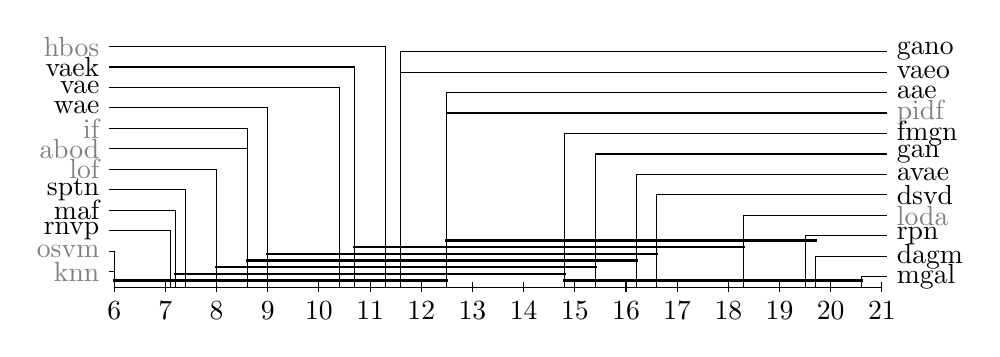
\begin{tikzpicture}[scale=0.65] 
  \draw (6.0,0) -- (21.0,0); 
  \foreach \x in {6,...,21} \draw (\x,0.10) -- (\x,-0.10) node[anchor=north]{$\x$}; 
  \draw (6.0,0) -- (6.0,0.30000000000000004) -- (5.9, 0.30000000000000004) node[anchor=east] {\textcolor{gray}{knn}}; 
  \draw (6.0,0) -- (6.0,0.7000000000000001) -- (5.9, 0.7000000000000001) node[anchor=east] {\textcolor{gray}{osvm}}; 
  \draw (7.1,0) -- (7.1,1.1) -- (5.9, 1.1) node[anchor=east] {rnvp}; 
  \draw (7.2,0) -- (7.2,1.5) -- (5.9, 1.5) node[anchor=east] {maf}; 
  \draw (7.4,0) -- (7.4,1.9) -- (5.9, 1.9) node[anchor=east] {sptn}; 
  \draw (8.0,0) -- (8.0,2.3000000000000003) -- (5.9, 2.3000000000000003) node[anchor=east] {\textcolor{gray}{lof}}; 
  \draw (8.6,0) -- (8.6,2.7) -- (5.9, 2.7) node[anchor=east] {\textcolor{gray}{abod}}; 
  \draw (8.6,0) -- (8.6,3.1) -- (5.9, 3.1) node[anchor=east] {\textcolor{gray}{if}}; 
  \draw (9.0,0) -- (9.0,3.5) -- (5.9, 3.5) node[anchor=east] {wae}; 
  \draw (10.4,0) -- (10.4,3.9) -- (5.9, 3.9) node[anchor=east] {vae}; 
  \draw (10.7,0) -- (10.7,4.300000000000001) -- (5.9, 4.300000000000001) node[anchor=east] {vaek}; 
  \draw (11.3,0) -- (11.3,4.700000000000001) -- (5.9, 4.700000000000001) node[anchor=east] {\textcolor{gray}{hbos}}; 
  \draw (11.6,0) -- (11.6,4.6000000000000005) -- (21.1, 4.6000000000000005) node[anchor=west] {gano}; 
  \draw (11.6,0) -- (11.6,4.2) -- (21.1, 4.2) node[anchor=west] {vaeo}; 
  \draw (12.5,0) -- (12.5,3.8000000000000003) -- (21.1, 3.8000000000000003) node[anchor=west] {aae}; 
  \draw (12.5,0) -- (12.5,3.4000000000000004) -- (21.1, 3.4000000000000004) node[anchor=west] {\textcolor{gray}{pidf}}; 
  \draw (14.8,0) -- (14.8,3.0000000000000004) -- (21.1, 3.0000000000000004) node[anchor=west] {fmgn}; 
  \draw (15.4,0) -- (15.4,2.6000000000000005) -- (21.1, 2.6000000000000005) node[anchor=west] {gan}; 
  \draw (16.2,0) -- (16.2,2.2) -- (21.1, 2.2) node[anchor=west] {avae}; 
  \draw (16.6,0) -- (16.6,1.8) -- (21.1, 1.8) node[anchor=west] {dsvd}; 
  \draw (18.3,0) -- (18.3,1.4000000000000001) -- (21.1, 1.4000000000000001) node[anchor=west] {\textcolor{gray}{loda}}; 
  \draw (19.5,0) -- (19.5,1.0) -- (21.1, 1.0) node[anchor=west] {rpn}; 
  \draw (19.7,0) -- (19.7,0.6000000000000001) -- (21.1, 0.6000000000000001) node[anchor=west] {dagm}; 
  \draw (20.6,0) -- (20.6,0.2) -- (21.1, 0.2) node[anchor=west] {mgal}; 
  \draw[line width=0.03cm,color=black,draw opacity=1.0] (5.97,0.13) -- (12.53,0.13); 
  \draw[line width=0.03cm,color=black,draw opacity=1.0] (7.17,0.26) -- (14.83,0.26); 
  \draw[line width=0.03cm,color=black,draw opacity=1.0] (7.97,0.39) -- (15.43,0.39); 
  \draw[line width=0.03cm,color=black,draw opacity=1.0] (8.57,0.52) -- (16.23,0.52); 
  \draw[line width=0.03cm,color=black,draw opacity=1.0] (8.97,0.65) -- (16.630000000000003,0.65); 
  \draw[line width=0.03cm,color=black,draw opacity=1.0] (10.67,0.78) -- (18.330000000000002,0.78); 
  \draw[line width=0.03cm,color=black,draw opacity=1.0] (12.47,0.91) -- (19.73,0.91); 
  \draw[line width=0.03cm,color=black,draw opacity=1.0] (14.770000000000001,0.13) -- (20.630000000000003,0.13); 
 \end{tikzpicture} 
} \\
    a) tabular datasets, anomaly validation & b) tabular datasets, clean validation \\  
    \resizebox{\columnwidth}{!}{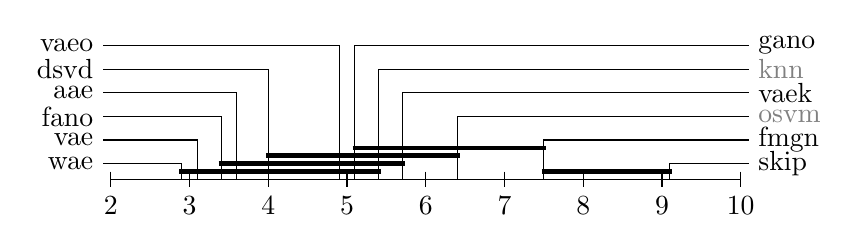
\begin{tikzpicture}[scale=1.0] 
  \draw (2.0,0) -- (10.0,0); 
  \foreach \x in {2,...,10} \draw (\x,0.10) -- (\x,-0.10) node[anchor=north]{$\x$}; 
  \draw (2.9,0) -- (2.9,0.19999999999999998) -- (1.9, 0.19999999999999998) node[anchor=east] {wae}; 
  \draw (3.1,0) -- (3.1,0.5) -- (1.9, 0.5) node[anchor=east] {vae}; 
  \draw (3.4,0) -- (3.4,0.7999999999999999) -- (1.9, 0.7999999999999999) node[anchor=east] {fano}; 
  \draw (3.6,0) -- (3.6,1.0999999999999999) -- (1.9, 1.0999999999999999) node[anchor=east] {aae}; 
  \draw (4.0,0) -- (4.0,1.4) -- (1.9, 1.4) node[anchor=east] {dsvd}; 
  \draw (4.9,0) -- (4.9,1.6999999999999997) -- (1.9, 1.6999999999999997) node[anchor=east] {vaeo}; 
  \draw (5.1,0) -- (5.1,1.7) -- (10.1, 1.7) node[anchor=west] {gano}; 
  \draw (5.4,0) -- (5.4,1.4) -- (10.1, 1.4) node[anchor=west] {\textcolor{gray}{knn}}; 
  \draw (5.7,0) -- (5.7,1.0999999999999999) -- (10.1, 1.0999999999999999) node[anchor=west] {vaek}; 
  \draw (6.4,0) -- (6.4,0.8) -- (10.1, 0.8) node[anchor=west] {\textcolor{gray}{osvm}}; 
  \draw (7.5,0) -- (7.5,0.5) -- (10.1, 0.5) node[anchor=west] {fmgn}; 
  \draw (9.1,0) -- (9.1,0.2) -- (10.1, 0.2) node[anchor=west] {skip}; 
  \draw[line width=0.06cm,color=black,draw opacity=1.0] (2.87,0.1) -- (5.430000000000001,0.1); 
  \draw[line width=0.06cm,color=black,draw opacity=1.0] (3.37,0.2) -- (5.73,0.2); 
  \draw[line width=0.06cm,color=black,draw opacity=1.0] (3.97,0.30000000000000004) -- (6.430000000000001,0.30000000000000004); 
  \draw[line width=0.06cm,color=black,draw opacity=1.0] (5.069999999999999,0.4) -- (7.53,0.4); 
  \draw[line width=0.06cm,color=black,draw opacity=1.0] (7.47,0.1) -- (9.129999999999999,0.1); 
 \end{tikzpicture} 
} & \resizebox{\columnwidth}{!}{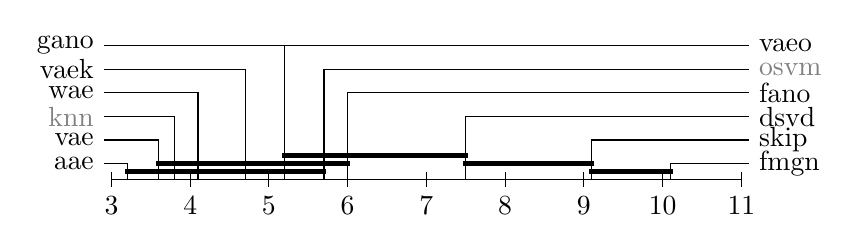
\begin{tikzpicture}[scale=1.0] 
  \draw (3.0,0) -- (11.0,0); 
  \foreach \x in {3,...,11} \draw (\x,0.10) -- (\x,-0.10) node[anchor=north]{$\x$}; 
  \draw (3.2,0) -- (3.2,0.19999999999999998) -- (2.9, 0.19999999999999998) node[anchor=east] {aae}; 
  \draw (3.6,0) -- (3.6,0.5) -- (2.9, 0.5) node[anchor=east] {vae}; 
  \draw (3.8,0) -- (3.8,0.7999999999999999) -- (2.9, 0.7999999999999999) node[anchor=east] {\textcolor{gray}{knn}}; 
  \draw (4.1,0) -- (4.1,1.0999999999999999) -- (2.9, 1.0999999999999999) node[anchor=east] {wae}; 
  \draw (4.7,0) -- (4.7,1.4) -- (2.9, 1.4) node[anchor=east] {vaek}; 
  \draw (5.2,0) -- (5.2,1.6999999999999997) -- (2.9, 1.6999999999999997) node[anchor=east] {gano}; 
  \draw (5.2,0) -- (5.2,1.7) -- (11.1, 1.7) node[anchor=west] {vaeo}; 
  \draw (5.7,0) -- (5.7,1.4) -- (11.1, 1.4) node[anchor=west] {\textcolor{gray}{osvm}}; 
  \draw (6.0,0) -- (6.0,1.0999999999999999) -- (11.1, 1.0999999999999999) node[anchor=west] {fano}; 
  \draw (7.5,0) -- (7.5,0.8) -- (11.1, 0.8) node[anchor=west] {dsvd}; 
  \draw (9.1,0) -- (9.1,0.5) -- (11.1, 0.5) node[anchor=west] {skip}; 
  \draw (10.1,0) -- (10.1,0.2) -- (11.1, 0.2) node[anchor=west] {fmgn}; 
  \draw[line width=0.06cm,color=black,draw opacity=1.0] (3.1700000000000004,0.1) -- (5.73,0.1); 
  \draw[line width=0.06cm,color=black,draw opacity=1.0] (3.5700000000000003,0.2) -- (6.03,0.2); 
  \draw[line width=0.06cm,color=black,draw opacity=1.0] (5.17,0.30000000000000004) -- (7.53,0.30000000000000004); 
  \draw[line width=0.06cm,color=black,draw opacity=1.0] (7.47,0.2) -- (9.129999999999999,0.2); 
  \draw[line width=0.06cm,color=black,draw opacity=1.0] (9.07,0.1) -- (10.129999999999999,0.1); 
 \end{tikzpicture} 
}\\
    c) statistical image datasets, anomaly validation & d) statistical image  datasets, clean validation \\ 
     \resizebox{\columnwidth}{!}{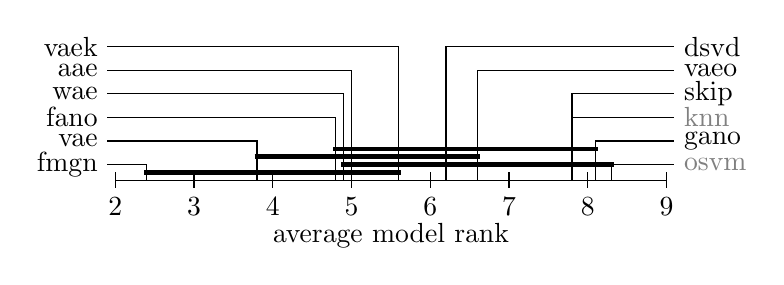
\begin{tikzpicture}[scale=1.0] 
  \draw (2.0,0) -- (9.0,0); 
  \foreach \x in {2,...,9} \draw (\x,0.10) -- (\x,-0.10) node[anchor=north]{$\x$}; 
  \draw (2.4,0) -- (2.4,0.19999999999999998) -- (1.9, 0.19999999999999998) node[anchor=east] {fmgn}; 
  \draw (3.8,0) -- (3.8,0.5) -- (1.9, 0.5) node[anchor=east] {vae}; 
  \draw (4.8,0) -- (4.8,0.7999999999999999) -- (1.9, 0.7999999999999999) node[anchor=east] {fano}; 
  \draw (4.9,0) -- (4.9,1.0999999999999999) -- (1.9, 1.0999999999999999) node[anchor=east] {wae}; 
  \draw (5.0,0) -- (5.0,1.4) -- (1.9, 1.4) node[anchor=east] {aae}; 
  \draw (5.6,0) -- (5.6,1.6999999999999997) -- (1.9, 1.6999999999999997) node[anchor=east] {vaek}; 
  \draw (6.2,0) -- (6.2,1.7) -- (9.1, 1.7) node[anchor=west] {dsvd}; 
  \draw (6.6,0) -- (6.6,1.4) -- (9.1, 1.4) node[anchor=west] {vaeo}; 
  \draw (7.8,0) -- (7.8,1.0999999999999999) -- (9.1, 1.0999999999999999) node[anchor=west] {skip}; 
  \draw (7.8,0) -- (7.8,0.8) -- (9.1, 0.8) node[anchor=west] {\textcolor{gray}{knn}}; 
  \draw (8.1,0) -- (8.1,0.5) -- (9.1, 0.5) node[anchor=west] {gano}; 
  \draw (8.3,0) -- (8.3,0.2) -- (9.1, 0.2) node[anchor=west] {\textcolor{gray}{osvm}}; 
  \draw[line width=0.06cm,color=black,draw opacity=1.0] (2.37,0.1) -- (5.63,0.1); 
  \draw[line width=0.06cm,color=black,draw opacity=1.0] (3.77,0.3) -- (6.63,0.3); 
  \draw[line width=0.06cm,color=black,draw opacity=1.0] (4.77,0.4) -- (8.129999999999999,0.4); 
  \draw[line width=0.06cm,color=black,draw opacity=1.0] (4.87,0.2) -- (8.33,0.2); 
  \node[anchor=center] at (5.5,-0.7) {average model rank};
 \end{tikzpicture} 
} & \resizebox{\columnwidth}{!}{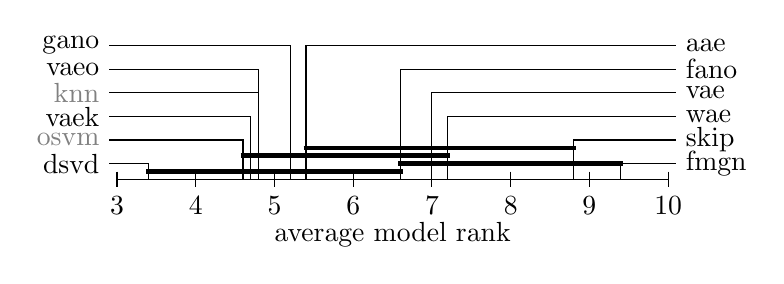
\begin{tikzpicture}[scale=1.0] 
  \draw (3.0,0) -- (10.0,0); 
  \foreach \x in {3,...,10} \draw (\x,0.10) -- (\x,-0.10) node[anchor=north]{$\x$}; 
  \draw (3.4,0) -- (3.4,0.19999999999999998) -- (2.9, 0.19999999999999998) node[anchor=east] {dsvd}; 
  \draw (4.6,0) -- (4.6,0.5) -- (2.9, 0.5) node[anchor=east] {\textcolor{gray}{osvm}}; 
  \draw (4.7,0) -- (4.7,0.7999999999999999) -- (2.9, 0.7999999999999999) node[anchor=east] {vaek}; 
  \draw (4.8,0) -- (4.8,1.0999999999999999) -- (2.9, 1.0999999999999999) node[anchor=east] {\textcolor{gray}{knn}}; 
  \draw (4.8,0) -- (4.8,1.4) -- (2.9, 1.4) node[anchor=east] {vaeo}; 
  \draw (5.2,0) -- (5.2,1.6999999999999997) -- (2.9, 1.6999999999999997) node[anchor=east] {gano}; 
  \draw (5.4,0) -- (5.4,1.7) -- (10.1, 1.7) node[anchor=west] {aae}; 
  \draw (6.6,0) -- (6.6,1.4) -- (10.1, 1.4) node[anchor=west] {fano}; 
  \draw (7.0,0) -- (7.0,1.0999999999999999) -- (10.1, 1.0999999999999999) node[anchor=west] {vae}; 
  \draw (7.2,0) -- (7.2,0.8) -- (10.1, 0.8) node[anchor=west] {wae}; 
  \draw (8.8,0) -- (8.8,0.5) -- (10.1, 0.5) node[anchor=west] {skip}; 
  \draw (9.4,0) -- (9.4,0.2) -- (10.1, 0.2) node[anchor=west] {fmgn}; 
  \draw[line width=0.06cm,color=black,draw opacity=1.0] (3.37,0.1) -- (6.63,0.1); 
  \draw[line width=0.06cm,color=black,draw opacity=1.0] (4.569999999999999,0.3) -- (7.23,0.3); 
  \draw[line width=0.06cm,color=black,draw opacity=1.0] (5.37,0.4) -- (8.83,0.4); 
  \draw[line width=0.06cm,color=black,draw opacity=1.0] (6.569999999999999,0.2) -- (9.43,0.2); 
  \node[anchor=center] at (6.5,-0.7) {average model rank};
 \end{tikzpicture} 
} \\
    e) semantic image  datasets, anomaly validation & f) semantic image datasets, clean validation \\
    \end{tabular}
 \caption{Critical difference diagram of models ranked via the test AUC. Models whose performance is statistically indistinguishable have a difference of ranks under the critical value of the Nemenyi test $CD_{0.1}$ and are joined by a horizontal band. Results are presented for different types of datasets: tabular (Top row), image datasets with statistical anomalies (Middle row), and image datasets with semantic anomalies (Bottom row); and two different hyperparameter selection cases: using anomalies in validation (left) and using clean validation (right).
 }
 % $CD_{0.05}(24, 40) = 5.75$
 \label{fig:critical_diag}
\end{figure*}

\subsection{Dataset context}
\label{sec:dataset_context}
The results of experimental comparison on all dataset types are presented in the form of critical difference diagrams (CDD) as recommended by Dem\v{s}ar~\cite{demvsar2006statistical}, are in Fig.~\ref{fig:critical_diag}. Diagrams show the average rank of detectors across the datasets together with a confidence band that indicates that a statistical test cannot reject the hypothesis that two detectors perform the same. The underlying  AUC values on the testing set for all individual datasets are given in Tab.~\ref{tab:tabular_anomalies}, \ref{tab:tabular_clean}, \ref{tab:images_stat_auc_auc_combined}, and~\ref{tab:images_semantic_auc_auc_combined}. We now comment on the influence of the datatype with respect to two types of hyperparameter selection strategies differing in the number of anomalies in the validation set as defined in Section~\ref{sec:contexts}: i) anomaly validation context, and ii) clean validation context.

\emph{Tabular data:} OC-SVM works the best and it is \emph{statistically better} than almost all detectors except autoencoder-based generative models and VAE combined with OC-SVM in the case of anomaly validation context. The first 11 places (roughly one half) belong to models that can be divided into three groups: (i) OC-SVM and its variants, which estimate a density level of a distribution; (ii) flow models and kNN, which estimate the pdf (un-normalized in case of kNN); (iii) and variants of auto-encoders, where reconstruction error is related to pdf as explained in~\cite{vsmidl2019anomaly}. The same types of methods occupy the top positions in the clean validation context, Fig.~\ref{fig:critical_diag}b), however in a different order. The best is the kNN, and all other pdf-modeling methods (flows) have improved relative to the anomaly validation context. The autoencoder-based methods moved beyond classical methods (LOF, ABOD, IF). We believe that models in the lower half of the scale in both validation contexts are not suitable for detecting statistical anomalies. We cannot explain the poor performance of MOGAAL, DAGMM, and adVAE,\footnote{We have contacted the author of pyOD from wherein we took the implementation of MOGAAL, and we were assured that his implementation is a copy of that provided by the authors. Therefore, we consider the implementation to be correct.} and we attribute it to different experimental environment. DeepSVDD was primarily implemented for image problems, where it performs relatively well.

Moreover, differences in mean ranks of many models in Fig.~\ref{fig:critical_diag} are statistically insignificant at level $p=0.1$, which is disappointing. Assuming the ranks remain the same, another 51 datasets would be needed to make the difference between OC-SVM and VAE statistically significant on tabular data with 50\% anomalies. This indicates that the results are still noisy and can be easily changed for a different choice of datasets.

\emph{Statistical image data:} WAE and VAE models have the best average rank when evaluated on statistical image data, although their lead is not statistically significant over most of the other models as is evident from Fig.~\ref{fig:critical_diag}c). The autoencoder-based methods (AAE,VAE,WAE) perform well also in the clean validation context, complemented by kNN, Fig.~\ref{fig:critical_diag}d).

\emph{Semantic image data}
A different story is told by Fig.~\ref{fig:critical_diag}e) where the ranking of methods on image datasets with semantic anomalies is dominated by fmGAN by a large margin in the anomaly validation context. However, it is also the worst method in the clean validation context. In an opposite manner, 
OC-SVM and kNN perform very poorly in the anomaly validation context, but they are among the best in the clean validation context.  The best performing method in the clean validation context is DeepSVDD~\cite{ruff2018deep}. We conjecture that the performance of the fmGAN is related to the variability of its training. With a sufficient number of anomalies in the validation set, it is possible to find one trained model that fits the problem.

The typical anomalies detected by various methods on image datasets are provided in the Supplementary \ref{sec:appendix_extending_image_results}.


\subsection{Hyperparameter selection context}
\label{sec:hyperparameter_context}
The influence of the hyperparameter selection procedure on the results in the previous section is now studied in detail for few selected methods. We choose only those that scored among the best in the previous section. First, we analyze the sensitivity of these methods to the number of anomalies in the validation set. Second, we study hyperparameter selection for two individual methods, variational autoencoder family and OC-SVM.

\subsubsection{Impact of the number of anomalies in the validation set}
\begin{figure*}[hbt!]
    \centering
    % \footnotesize
    % \resizebox {\linewidth}{!}{
    % \input{data/chapter_comparison/combined_knowledge_rank_pat_auc_repre_mvc}
    % \input{data/chapter_comparison/combined_knowledge_rank_pat_auc_repre_mvc_per_ac}
    \begin{tikzpicture}[]
\begin{groupplot}[group style={vertical sep = 0.5cm, horizontal sep = 1.0cm, group size=3 by 1}]

\nextgroupplot [
  % legend style = {at={(0.3,1.30)}, anchor=west},
  ylabel = {avg. AUC},
  width=5cm, height=7cm, scale only axis=true, 
  xtick={1,2,3,4,5,6,7,8}, 
  xticklabels={clean,$PR@\%0.01$,$PR@\%0.1$,$PR@\%1$,$PR@\%5$,$PR@\%10$,$PR@\%20$,$AUC_{val}$},
  width=5cm, height=7cm, scale only axis=true,
  x tick label style={rotate=50,anchor=east},
  title = {(tabular)},
  % title style={at={(current bounding box.north)}, anchor=west},
]

\addplot+ coordinates {
  (1.0, 0.72375)
  (2.0, 0.762)
  (3.0, 0.754)
  (4.0, 0.8047500000000001)
  (5.0, 0.83925)
  (6.0, 0.844)
  (7.0, 0.8562500000000002)
  (8.0, 0.8845000000000001)
};

\addplot+ coordinates {
  (1.0, 0.607)
  (2.0, 0.52475)
  (3.0, 0.5587500000000001)
  (4.0, 0.5867500000000001)
  (5.0, 0.6585)
  (6.0, 0.71375)
  (7.0, 0.7232500000000001)
  (8.0, 0.7502500000000001)
};

\addplot+ coordinates {};

\addplot+ coordinates {
  (1.0, 0.6375)
  (2.0, 0.66375)
  (3.0, 0.6797500000000001)
  (4.0, 0.6940000000000001)
  (5.0, 0.75325)
  (6.0, 0.7837500000000001)
  (7.0, 0.8067500000000001)
  (8.0, 0.8380000000000001)
};

\addplot+ coordinates {
  (1.0, 0.8087500000000002)
  (2.0, 0.8290000000000001)
  (3.0, 0.8310000000000001)
  (4.0, 0.8329999999999999)
  (5.0, 0.8362499999999999)
  (6.0, 0.8357499999999998)
  (7.0, 0.8454999999999998)
  (8.0, 0.8517499999999998)
};

\addplot+ coordinates {
  (1.0, 0.8145)
  (2.0, 0.7222500000000001)
  (3.0, 0.7222500000000001)
  (4.0, 0.77225)
  (5.0, 0.8247500000000001)
  (6.0, 0.8727499999999999)
  (7.0, 0.8854999999999998)
  (8.0, 0.9112500000000001)
};

\addplot+ coordinates {
  (1.0, 0.7329999999999999)
  (2.0, 0.7945)
  (3.0, 0.7665)
  (4.0, 0.7812500000000001)
  (5.0, 0.8154999999999999)
  (6.0, 0.8247499999999999)
  (7.0, 0.8310000000000001)
  (8.0, 0.8714999999999999)
};

\addplot+ coordinates {
  (1.0, 0.7372500000000001)
  (2.0, 0.5530000000000002)
  (3.0, 0.5897500000000002)
  (4.0, 0.6622499999999999)
  (5.0, 0.7882499999999999)
  (6.0, 0.79475)
  (7.0, 0.84175)
  (8.0, 0.8825)
};

\addplot+ coordinates {
  (1.0, 0.7842499999999999)
  (2.0, 0.7955000000000002)
  (3.0, 0.7945)
  (4.0, 0.79525)
  (5.0, 0.826)
  (6.0, 0.836)
  (7.0, 0.853)
  (8.0, 0.8647499999999999)
};

\addplot+ coordinates {
  (1.0, 0.7967500000000001)
  (2.0, 0.7994999999999999)
  (3.0, 0.8039999999999999)
  (4.0, 0.7997500000000002)
  (5.0, 0.8217500000000001)
  (6.0, 0.82675)
  (7.0, 0.8344999999999999)
  (8.0, 0.8482500000000002)
};

% \legend{{}{aae}, {}{dsvd}, {}{fmgn}, {}{knn}, {}{osvm}, {}{vae}, {}{vaeo}, {}{wae}, {}{rnvp}}

\nextgroupplot [
  legend columns = -1,
  legend style = {at={(0.5,1.2)}, anchor=center},
  legend entries = {aae, dsvd, fano, fmgn, knn, osvm, vae, vaeo, wae, rnvp},
  width=5cm, height=7cm, scale only axis=true, 
  xtick={1,2,3,4,5,6,7,8}, 
  xticklabels={clean,$PR@\%0.01$,$PR@\%0.1$,$PR@\%1$,$PR@\%5$,$PR@\%10$,$PR@\%20$,$AUC_{val}$},
  width=5cm, height=7cm, scale only axis=true,
  x tick label style={rotate=50,anchor=east},
  title = {(statistical)},
  % title style={at={(current bounding box.north)}, anchor=west},
]

\addplot+ coordinates {
  (1.0, 0.8664864864864865)
  (2.0, 0.867837837837838)
  (3.0, 0.8791891891891892)
  (4.0, 0.8999999999999999)
  (5.0, 0.8981081081081083)
  (6.0, 0.8978378378378378)
  (7.0, 0.901891891891892)
  (8.0, 0.908918918918919)
};

\addplot+ coordinates {
  (1.0, 0.654054054054054)
  (2.0, 0.7918918918918918)
  (3.0, 0.8108108108108109)
  (4.0, 0.8327027027027026)
  (5.0, 0.841891891891892)
  (6.0, 0.8543243243243243)
  (7.0, 0.8597297297297297)
  (8.0, 0.8802702702702703)
};

\addplot+ coordinates {
  (1.0, 0.841891891891892)
  (2.0, 0.8527027027027027)
  (3.0, 0.8589189189189189)
  (4.0, 0.8727027027027027)
  (5.0, 0.8891891891891893)
  (6.0, 0.8959459459459459)
  (7.0, 0.9045945945945946)
  (8.0, 0.9275675675675675)
};

\addplot+ coordinates {
  (1.0, 0.5199999999999999)
  (2.0, 0.5445945945945946)
  (3.0, 0.5948648648648649)
  (4.0, 0.6775675675675675)
  (5.0, 0.73)
  (6.0, 0.7454054054054053)
  (7.0, 0.8075675675675675)
  (8.0, 0.8856756756756757)
};

\addplot+ coordinates {
  (1.0, 0.8262162162162162)
  (2.0, 0.8670270270270269)
  (3.0, 0.8708108108108108)
  (4.0, 0.8781081081081081)
  (5.0, 0.8781081081081081)
  (6.0, 0.8783783783783784)
  (7.0, 0.8799999999999999)
  (8.0, 0.8856756756756757)
};

\addplot+ coordinates {
  (1.0, 0.7997297297297298)
  (2.0, 0.7021621621621621)
  (3.0, 0.7032432432432432)
  (4.0, 0.7451351351351351)
  (5.0, 0.7983783783783783)
  (6.0, 0.8308108108108109)
  (7.0, 0.8394594594594594)
  (8.0, 0.8824324324324324)
};

\addplot+ coordinates {
  (1.0, 0.8856756756756757)
  (2.0, 0.7954054054054054)
  (3.0, 0.8127027027027027)
  (4.0, 0.828918918918919)
  (5.0, 0.8727027027027027)
  (6.0, 0.897027027027027)
  (7.0, 0.905945945945946)
  (8.0, 0.9205405405405408)
};

\addplot+ coordinates {
  (1.0, 0.8164864864864865)
  (2.0, 0.687027027027027)
  (3.0, 0.6967567567567567)
  (4.0, 0.7478378378378379)
  (5.0, 0.851081081081081)
  (6.0, 0.8794594594594595)
  (7.0, 0.9013513513513514)
  (8.0, 0.929189189189189)
};

\addplot+ coordinates {
  (1.0, 0.8916216216216215)
  (2.0, 0.8862162162162162)
  (3.0, 0.8986486486486487)
  (4.0, 0.8997297297297298)
  (5.0, 0.9183783783783783)
  (6.0, 0.9205405405405406)
  (7.0, 0.9224324324324323)
  (8.0, 0.9289189189189189)
};

% has to be set manually to match the marker style of the flow (9th in the entries bellow)
\addlegendimage{red,densely dashed,every mark/.append style={solid,fill=red!80!black},mark=diamond*} 
% \legend{{}{aae}, {}{dsvd}, {}{fano}, {}{fmgn}, {}{knn}, {}{osvm}, {}{vae}, {}{vaeo}, {}{wae}}

%%% the color 
% blue,every mark/.append style={fill=blue!80!black},mark=*\\
% red,every mark/.append style={fill=red!80!black},mark=square*\\
% brown!60!black,every mark/.append style={fill=brown!80!black},mark=otimes*\\
% black,mark=star\\
% blue,every mark/.append style={fill=blue!80!black},mark=diamond*\\
% red,densely dashed,every mark/.append style={solid,fill=red!80!black},mark=*\\
% brown!60!black,densely dashed,every mark/.append style={
% solid,fill=brown!80!black},mark=square*\\
% black,densely dashed,every mark/.append style={solid,fill=gray},mark=otimes*\\
% blue,densely dashed,mark=star,every mark/.append style=solid\\
% red,densely dashed,every mark/.append style={solid,fill=red!80!black},mark=diamond*\\

\nextgroupplot [
  % legend style = {at={(0.3,1.30)}, anchor=west},
  width=5cm, height=7cm, scale only axis=true, 
  xtick={1,2,3,4,5,6,7,8}, 
  xticklabels={clean,$PR@\%0.01$,$PR@\%0.1$,$PR@\%1$,$PR@\%5$,$PR@\%10$,$PR@\%20$,$AUC_{val}$},
  width=5cm, height=7cm, scale only axis=true,
  x tick label style={rotate=50,anchor=east},
  title = {(semantic)},
  % title style={at={(current bounding box.north)}, anchor=west},
]

\addplot+ coordinates {
  (1.0, 0.5649999999999998)
  (2.0, 0.584)
  (3.0, 0.5745000000000001)
  (4.0, 0.5934999999999999)
  (5.0, 0.6)
  (6.0, 0.6079999999999999)
  (7.0, 0.614)
  (8.0, 0.6224999999999999)
};

\addplot+ coordinates {
  (1.0, 0.5920000000000001)
  (2.0, 0.575)
  (3.0, 0.5685)
  (4.0, 0.5975000000000001)
  (5.0, 0.6250000000000001)
  (6.0, 0.6320000000000001)
  (7.0, 0.6325000000000001)
  (8.0, 0.638)
};

\addplot+ coordinates {
  (1.0, 0.5595000000000001)
  (2.0, 0.541)
  (3.0, 0.5544999999999999)
  (4.0, 0.5899999999999999)
  (5.0, 0.5955)
  (6.0, 0.61)
  (7.0, 0.633)
  (8.0, 0.6424999999999998)
};

\addplot+ coordinates {
  (1.0, 0.5)
  (2.0, 0.4885)
  (3.0, 0.49799999999999994)
  (4.0, 0.6194999999999999)
  (5.0, 0.6765)
  (6.0, 0.7)
  (7.0, 0.7249999999999999)
  (8.0, 0.729)
};

\addplot+ coordinates {
  (1.0, 0.5730000000000001)
  (2.0, 0.5834999999999999)
  (3.0, 0.5824999999999999)
  (4.0, 0.5890000000000001)
  (5.0, 0.5945)
  (6.0, 0.5985)
  (7.0, 0.599)
  (8.0, 0.6015)
};

\addplot+ coordinates {
  (1.0, 0.5760000000000001)
  (2.0, 0.5090000000000001)
  (3.0, 0.536)
  (4.0, 0.5625)
  (5.0, 0.5860000000000001)
  (6.0, 0.5925)
  (7.0, 0.5975000000000001)
  (8.0, 0.6045)
};

\addplot+ coordinates {
  (1.0, 0.552)
  (2.0, 0.5469999999999999)
  (3.0, 0.5625)
  (4.0, 0.5995000000000001)
  (5.0, 0.6210000000000002)
  (6.0, 0.6315000000000001)
  (7.0, 0.6315)
  (8.0, 0.6439999999999999)
};

\addplot+ coordinates {
  (1.0, 0.5735000000000001)
  (2.0, 0.558)
  (3.0, 0.5574999999999999)
  (4.0, 0.574)
  (5.0, 0.588)
  (6.0, 0.5994999999999999)
  (7.0, 0.6035000000000001)
  (8.0, 0.619)
};

\addplot+ coordinates {
  (1.0, 0.549)
  (2.0, 0.5820000000000002)
  (3.0, 0.5705)
  (4.0, 0.6065)
  (5.0, 0.614)
  (6.0, 0.615)
  (7.0, 0.625)
  (8.0, 0.6305)
};

\end{groupplot}

\end{tikzpicture}

    % }
    \caption{Sensitivity of methods to the number of anomalies available in the validation set for hyperparameter selection visualized in terms of the achieved AUC aggregated over all datasets in each category (columns). The clean validation context is the left-most point on the x-axis, and the anomaly validation context (50\% of available anomalies) is the right-most point. The points in-between were obtained by selecting models with the highest precision on the reported portion (e.g. 5\%) of validation samples with the highest anomaly scores.} 
    \label{fig:combined_knowledge_rank_patn_auc_repre}
\end{figure*}

The process of hyperparameter selection described in Sec.~\ref{sub:hyperparameteroptimization} depends on the availability of examples of anomalies in the validation set (recall that it is assumed that the validation dataset does not contain unknown anomalous samples, i.e. is not contaminated). 
Fig.~\ref{fig:combined_knowledge_rank_patn_auc_repre} displays the influence of the number of anomalous samples in the validation set on a finer grid between the two contexts reported before.  Note that for the first point on the x-axis, \textit{clean}, the mechanism of model selection was different from the rest of the graph, as noted in Sec.~\ref{sub:hyperparameteroptimization}. This is the reason for the significant difference between the clean context and the remaining points.

First, we observe that the quality of the models selected using anomalies improves with an increasing number of anomalous samples which is expected. However, for a low number of anomalies, many methods perform significantly worse than in the case of the clean validation context. This behavior is notable across dataset types, especially for OC-SVM, and to some extent VAE. We conjecture that the hyperparameter selection procedure of those methods has a tendency to overfit, and its hyperparameters are not robust. In contrast to this, the performance of kNN, WAE, and RealNVP degrades slowly with the declining number of anomalies, which suggests that they are quite robust in difficult operating conditions. We attribute it to the fact that these methods are more exact in their estimation of data likelihood than the rest. 

Second, we notice that the experimental results on the semantic image datasets are generally poor, as the AUC of the best model (fmGAN) on CIFAR10 is 0.72 and similarly on SVHN2, where the best model achieved $0.74$. On the other hand, anomaly detection methods perform well on statistical image datasets. This indicates, contrary to popular belief that the models fail to learn or identify the important semantic information, or they consider different semantic information anomalous, and they should be told \emph{which} semantic aspect of an image should be considered as an anomaly, as for example blurred images might be anomalous as well.

Results of the same study for individual image datasets are presented in the Supplementary, Fig.~\ref{fig:image_knowledge_rank_pat_auc}. We also provide an illustration of what images were identified as normal and anomalous for the tested methods, Supplementary~\ref{sec:appendix_extending_image_results}.

A practitioner might also desire a method robust with respect to a poor choice of hyperparameters.  In general, deep methods in our experiments have demonstrated higher variance, probably due to the large number of hyperparameters and stochasticity involved in their initialization and training via batched gradient optimization. In this respect, GAN-based models seem to be the least robust, which is in line with~\cite{deecke2018image} stating that GANs are not directly optimized for anomaly detection. This hints at the potential cost of hyperparameter optimization --- with higher performance variance, one is less likely to train a well-performing model in a given number of attempts. 

\subsubsection{Sensitivity Analysis of the VAE family}
\label{sec:vae_results}
Autoencoder-based methods form a whole family with multiple sources of variability, as identified in Sec.~\ref{sec:ae_theory} to be: i) approximation of the likelihood in training (loss function), ii) the richness of latent prior, and iii) the anomaly score. We will analyze the sensitivity of the results to these choices on tabular data in the anomaly validation context. We focus on this family since most of the novel deep generative models for anomaly detection are based on the autoencoder architecture. Additional degrees of freedom include the parametrization of variance of $p_{\vec{\theta}}(\vec{x}|\vec{z}),$ which could be either fixed (called VAE-constant), used in~\cite{yaoUnsupervisedAnomalyDetection2019, wang2020advae, ahnDeepGenerativeModelsBased2020}, scalar (called VAE-scalar), or full diagonal (called VAE-diagonal), used in~\cite{an2015variational,xu2018unsupervised, zenatiEfficientGANBasedAnomaly2018}. In the experiments, all three variations were tested on tabular data; however on image data, the full diagonal was skipped due to computational constraints (and in line with the prior art, where only fixed variance is used).

The overall comparison in Fig.~\ref{fig:critical_diag} revealed that WAE and vanilla VAE variants perform best. The other degrees of freedom, namely richness of prior, used anomaly score, and parametrization of variance, were treated as hyperparameters. Fig.~\ref{fig:tabular_ae_only_box_auc_meanmax} extends the study by showing the distribution of ranks over tabular datasets for different variants of VAE, including GANomaly and adVAE.

First, notice that the spread of the method's ranks over various datasets is significant, as even ranks of the best methods vary from 3 to 15. This means that the conclusions below need to be taken with a grain of salt, as the experimental results are extremely noisy.

The ELBO-based score,  -el, together with the orthogonal decomposition of the likelihood~\cite{pidhorskyi2018generative}, -jc, does not perform well. The sampled reconstruction error (an MC estimate of~\eqref{eq:score_sample}, \mbox{-rs}, almost always performs better than the usual reconstruction error, -rm, calculated according to~\eqref{eq:score_mean}. This demonstrates that the common approach of replacing the mean of the decoder with that of the encoder is inferior but computationally cheaper (see Tab.~\ref{tab:predict_times} with prediction times). The discriminator score~\eqref{eq:disc_score}, -di, of AAE (an autoencoder combined with GAN) seems to be also on par with the MC estimate~\eqref{eq:score_sample}. 

From the same figure, we also conclude that the models modelling full diagonal in $p_{\vec{\theta}}(\vec{x}|\vec{z})$, -d-, seem to be better than the scalar, -s-, or constant, -c-, variants. This result is important, as many comparisons in the prior art use the VAE-constant, despite the version with full diagonal being discussed in the original publication~\cite{kingma2013auto}.

The rich prior distribution on the latent space proposed in \cite{tomczak2018vae}, VAMP, -v-, does not seem to give an advantage in the anomaly detection except in the AAE. Similarly, recent variants adVAE and GANomaly do not seem to work well on the tabular data, but they were not evaluated on them in the original publications.

\begin{figure}
    \centering
    \small
    % \input{data/chapter_comparison/tabular_ae_only_box_auc_meanmax}
    \begin{tikzpicture}
\begin{axis}[
	height=12cm,
	width=8cm,
	ymin=0, ymax=47,
	xmin=0, xmax=35,
	ytick={1,3,5,6,7,8,10,11,12,14,15,16,18,19,20,22,23,24,25,27,28,29,31,32,33,35,36,37,39,40,42,43,45,46},
	yticklabels={avae,gano,aae-s-di,aae-s-jc,aae-s-rm,aae-s-rs,aae-sv-di,aae-sv-rm,aae-sv-rs,aae-d-di,aae-d-rm,aae-d-rs,aae-dv-di,aae-dv-rm,aae-dv-rs,vae-s-el,vae-s-jc,vae-s-rm,vae-s-rs,vae-d-el,vae-d-rm,vae-d-rs,vae-c-el,vae-c-rm,vae-c-rs,wae-s-jc,wae-s-rm,wae-s-rs,wae-sv-rm,wae-sv-rs,wae-d-rm,wae-d-rs,wae-dv-rm,wae-dv-rs}
	]
\addplot [fill=lightgray, boxplot prepared={
draw position=1,
lower whisker=34, lower quartile=13.75,
median=21.5, upper quartile=28.25,
upper whisker=34},
] coordinates {};
\addplot [fill=lightgray, boxplot prepared={
draw position=3,
lower whisker=34, lower quartile=3.75,
median=15.0, upper quartile=23.5,
upper whisker=34},
] coordinates {};
\addplot [fill=lime, boxplot prepared={
draw position=5,
lower whisker=30, lower quartile=6.0,
median=12.0, upper quartile=21.25,
upper whisker=30},
] coordinates {};
\addplot [fill=orange, boxplot prepared={
draw position=6,
lower whisker=34, lower quartile=11.5,
median=21.5, upper quartile=26.75,
upper whisker=34},
] coordinates {};
\addplot [fill=cyan, boxplot prepared={
draw position=7,
lower whisker=33, lower quartile=9.0,
median=16.5, upper quartile=24.25,
upper whisker=33},
] coordinates {};
\addplot [fill=red, boxplot prepared={
draw position=8,
lower whisker=31, lower quartile=6.0,
median=16.0, upper quartile=22.25,
upper whisker=31},
] coordinates {};
\addplot [fill=lime, boxplot prepared={
draw position=10,
lower whisker=32, lower quartile=7.75,
median=12.5, upper quartile=22.25,
upper whisker=32},
] coordinates {};
\addplot [fill=cyan, boxplot prepared={
draw position=11,
lower whisker=34, lower quartile=8.75,
median=15.0, upper quartile=21.75,
upper whisker=34},
] coordinates {};
\addplot [fill=red, boxplot prepared={
draw position=12,
lower whisker=31, lower quartile=5.0,
median=12.0, upper quartile=21.25,
upper whisker=31},
] coordinates {};
\addplot [fill=lime, boxplot prepared={
draw position=14,
lower whisker=34, lower quartile=5.5,
median=23.0, upper quartile=32.0,
upper whisker=34},
] coordinates {};
\addplot [fill=cyan, boxplot prepared={
draw position=15,
lower whisker=31, lower quartile=12.75,
median=20.0, upper quartile=25.0,
upper whisker=31},
] coordinates {};
\addplot [fill=red, boxplot prepared={
draw position=16,
lower whisker=31, lower quartile=7.0,
median=14.5, upper quartile=21.25,
upper whisker=31},
] coordinates {};
\addplot [fill=lime, boxplot prepared={
draw position=18,
lower whisker=34, lower quartile=3.0,
median=26.0, upper quartile=33.25,
upper whisker=34},
] coordinates {};
\addplot [fill=cyan, boxplot prepared={
draw position=19,
lower whisker=33, lower quartile=10.75,
median=19.0, upper quartile=27.25,
upper whisker=33},
] coordinates {};
\addplot [fill=red, boxplot prepared={
draw position=20,
lower whisker=33, lower quartile=7.0,
median=15.0, upper quartile=25.25,
upper whisker=33},
] coordinates {};
\addplot [fill=magenta, boxplot prepared={
draw position=22,
lower whisker=32, lower quartile=5.0,
median=16.0, upper quartile=23.0,
upper whisker=32},
] coordinates {};
\addplot [fill=orange, boxplot prepared={
draw position=23,
lower whisker=33, lower quartile=11.5,
median=18.0, upper quartile=23.0,
upper whisker=33},
] coordinates {};
\addplot [fill=cyan, boxplot prepared={
draw position=24,
lower whisker=34, lower quartile=6.0,
median=12.5, upper quartile=23.0,
upper whisker=34},
] coordinates {};
\addplot [fill=red, boxplot prepared={
draw position=25,
lower whisker=31, lower quartile=3.0,
median=12.5, upper quartile=20.25,
upper whisker=31},
] coordinates {};
\addplot [fill=magenta, boxplot prepared={
draw position=27,
lower whisker=33, lower quartile=4.5,
median=9.0, upper quartile=22.0,
upper whisker=33},
] coordinates {};
\addplot [fill=cyan, boxplot prepared={
draw position=28,
lower whisker=33, lower quartile=2.0,
median=11.0, upper quartile=22.25,
upper whisker=33},
] coordinates {};
\addplot [fill=red, boxplot prepared={
draw position=29,
lower whisker=32, lower quartile=2.0,
median=5.5, upper quartile=20.0,
upper whisker=32},
] coordinates {};
\addplot [fill=magenta, boxplot prepared={
draw position=31,
lower whisker=34, lower quartile=10.5,
median=21.5, upper quartile=31.0,
upper whisker=34},
] coordinates {};
\addplot [fill=cyan, boxplot prepared={
draw position=32,
lower whisker=34, lower quartile=7.25,
median=9.0, upper quartile=18.25,
upper whisker=34},
] coordinates {};
\addplot [fill=red, boxplot prepared={
draw position=33,
lower whisker=33, lower quartile=7.75,
median=16.5, upper quartile=25.0,
upper whisker=33},
] coordinates {};
\addplot [fill=orange, boxplot prepared={
draw position=35,
lower whisker=34, lower quartile=11.25,
median=22.5, upper quartile=31.25,
upper whisker=34},
] coordinates {};
\addplot [fill=cyan, boxplot prepared={
draw position=36,
lower whisker=30, lower quartile=5.0,
median=11.5, upper quartile=18.25,
upper whisker=30},
] coordinates {};
\addplot [fill=red, boxplot prepared={
draw position=37,
lower whisker=33, lower quartile=3.0,
median=7.0, upper quartile=17.25,
upper whisker=33},
] coordinates {};
\addplot [fill=cyan, boxplot prepared={
draw position=39,
lower whisker=32, lower quartile=5.0,
median=10.0, upper quartile=20.25,
upper whisker=32},
] coordinates {};
\addplot [fill=red, boxplot prepared={
draw position=40,
lower whisker=31, lower quartile=3.0,
median=7.0, upper quartile=15.25,
upper whisker=31},
] coordinates {};
\addplot [fill=cyan, boxplot prepared={
draw position=42,
lower whisker=31, lower quartile=2.0,
median=7.5, upper quartile=18.0,
upper whisker=31},
] coordinates {};
\addplot [fill=red, boxplot prepared={
draw position=43,
lower whisker=31, lower quartile=2.0,
median=6.0, upper quartile=15.75,
upper whisker=31},
] coordinates {};
\addplot [fill=cyan, boxplot prepared={
draw position=45,
lower whisker=33, lower quartile=6.0,
median=10.5, upper quartile=17.25,
upper whisker=33},
] coordinates {};
\addplot [fill=red, boxplot prepared={
draw position=46,
lower whisker=33, lower quartile=3.0,
median=7.0, upper quartile=13.0,
upper whisker=33},
] coordinates {};
\end{axis}
\end{tikzpicture}

    \caption{Sensitivity study of various variants of  autoencoder-based methods displayed in the form of boxplots of their ranks in the AUC metric achieved on the tabular datasets. The first three letters of the method's name denote the training loss. Models with the -d- middle part estimate full diagonal of the decoder variance, -s- estimate only a scalar, and -c-  use a fixed scalar variance as a hyperparameter. All variants are using the standard Gaussian latent model. Models using the VampPrior are denoted by extending the decoder variance symbol by the letter v-, i.e. -dv-, -sv-, -cv-. The last part of the name denotes score, -rs stands for the sampled rec. probability~\eqref{eq:score_sample} with $L=100$, -rm for~\eqref{eq:score_mean}, -el for the ELBO~\eqref{eq:vae_loss} composed of -rs and KLD, -jc for~\eqref{eq:jacodeco}, -di for~\eqref{eq:disc_score}.}
    \label{fig:tabular_ae_only_box_auc_meanmax}
\end{figure}


\begin{table}
    \footnotesize
    \centering
    \tabcolsep=0.05cm
    \begin{tabular}{c|c c c c c}
         & vae-s-rs & vae-d-rs & vae-s-rm & vae-d-rm & vae-d-jc \\
         \midrule
        $\bar{t}_{pred}$ [s] & 12.10 & 18.51 & 0.11 & 0.15 & 57.31
    \end{tabular}
    \vspace*{0.15cm}
    \caption{Average prediction times on the  tabular datasets for different combinations of VAE scores and decoder variance estimations. The -d- part stands for model with an estimate of the full diagonal of the decoder variance, -s- is a scalar estimate. Sampled reconstruction error~\eqref{eq:score_sample} is denoted as -rs, -rm is the anomaly score~\eqref{eq:score_mean} and -jc is~\eqref{eq:jacodeco}.}
    \label{tab:predict_times}
\end{table}



\subsubsection{Sensitivity study of OC-SVM}
\label{sub:OC-SVM}
The domination of OC-SVM on tabular data in anomaly validation context contrasts to many prior experimental comparisons~\cite{goldstein2016comparative, chalapathyGroupAnomalyDetection2018, deecke2018image, gopalanPIDForestAnomalyDetection2019, iwataSupervisedAnomalyDetection2019, wang2020advae}. The search for the culprit found it to be the hyperparameter selection. This study has varied the $\nu$ parameter, kernels, and their parameters, which is much more than the most prior art does, which is fixing the kernel to RBF and tests few values of its width $\gamma$ and $\nu.$ Inclusion of other kernels into the search for hyperparameters seems to be the major source of improvement in this case. Replacing the OC-SVM with one restricted to use only the RBF kernel and $\nu=0.5$ yields an increase in average rank from $2.9$ to $8.1$ with an average decrease in performance by $0.06$, measured in AUC in the anomaly validation context. This version of OC-SVM is then easily surpassed by variational autoencoders and kNN, as demonstrated in Supplementary, Tab.~\ref{tab:tabular_auc_auc_meanmax_orbf_ranks_only}.  The importance of the choice of the kernel is furthermore illustrated by the fact that the sigmoid kernel was the optimal choice for 23 datasets, while the RBF kernel was optimal only for 13. Ref.~\cite{goldstein2016comparative} mentions that setting $\nu=0.5$ provides universally good results, which may be the reason why many authors do not tune it. In theory, it should be set to much lower values ($\nu = 0.05$) corresponding to the presumed low ratio of anomalies in data, but with Bayesian optimization, we found that the best estimate of $\nu$ was in some cases even higher, such as $\sim0.75$ on the statlog-vehicle dataset.

\subsection{Economic context}
\label{sec:economic_context}
\begin{figure*}
    \centering
    \begin{subfigure}{\columnwidth}
        \centering
        \small
        \resizebox {\linewidth}{!}{
            \begin{tikzpicture}[]
\begin{groupplot}[group style={vertical sep = 0.0cm, horizontal sep = 0.2cm, group size=2 by 1}]

\nextgroupplot [
  xlabel = {avg. rank},
  ylabel = {avg. training time rank},
  ylabel near ticks, yticklabel pos=left,
  ymin = 0.5, ymax=25,
  width=4cm, height=6cm, scale only axis=true,
  grid=major,
  % title = {(fit time)}
]

\addplot+[
  draw = none
] coordinates {
  (6.9, 11.3)
  (11.4, 8.8)
  (13.4, 12.7)
  (19.8, 16.2)
  (16.2, 10.9)
  (11.4, 18.8)
  (12.0, 16.2)
  (10.3, 9.7)
  (14.9, 4.4)
  (14.5, 5.0)
  (8.4, 2.4)
  (16.1, 3.4)
  (11.4, 2.6)
  (8.9, 21.8)
  % (22.3, 19.4)
  (2.9, 3.4)
  (14.3, 15.1)
  (9.0, 23.3)
  (12.1, 7.6)
  (10.7, 23.0)
  (6.5, 12.1)
  (11.0, 16.3)
  (6.8, 14.9)
  (7.0, 20.1)
};

\node at (axis cs:8.2, 12.0) {aae};

\node at (axis cs:13.1, 9.7) {abod};

\node at (axis cs:13.9, 13.3) {avae};

\node at (axis cs:18.9, 16.9) {dagm};

\node at (axis cs:16.7, 11.8) {dsvd};

\node at (axis cs:11.9, 19.5) {fmgn};

\node at (axis cs:13.0, 17.0) {gan};

\node at (axis cs:10.8, 10.3) {gano};

\node at (axis cs:16.8, 5.1) {hbos};

\node at (axis cs:14.1, 5.8) {if};

\node at (axis cs:8.8, 3.2) {knn};

\node at (axis cs:17.8, 2.9) {loda};

\node at (axis cs:11.6, 3.4) {lof};

\node at (axis cs:11.0, 21.8) {maf};

% \node at (axis cs:22.8, 20.0) {mgal};

\node at (axis cs:3.4, 4.1) {osvm};

\node at (axis cs:14.8, 15.7) {pidf};

\node at (axis cs:9.1, 24.0) {rnvp};

\node at (axis cs:13.6, 8.0) {rpn};

\node at (axis cs:12.8, 23.7) {sptn};

\node at (axis cs:7.0, 12.7) {vae};

\node at (axis cs:9.3, 17.0) {vaek};

\node at (axis cs:7.3, 15.6) {vaeo};

\node at (axis cs:7.5, 20.8) {wae};

\nextgroupplot [
  xlabel = {avg. rank},
  ylabel = {avg. prediction time rank},
  ylabel near ticks, yticklabel pos=right,
  ymin = 0.5, ymax=25,
  width=4cm, height=6cm, scale only axis=true,
  % title = {(evaluation time)},
  grid=major,
  % yticklabels={}
]

\addplot+[
  draw = none
] coordinates {
  (6.9, 13.3)    
  (11.4, 23.8)    
  (13.4, 21.8)
  (19.8, 1.3)
  (16.2, 7.0)
  (11.4, 2.3)
  (12.0, 2.2)
  (10.3, 5.6)
  (14.9, 4.4)
  (14.5, 16.0)
  (8.4, 15.1)
  (16.1, 10.4)
  (11.4, 11.5)
  (8.9, 12.2)
  % (22.3, 10.0)
  (2.9, 10.1)
  (14.3, 22.6)
  (9.0, 8.7)
  (12.1, 10.5)
  (10.7, 17.0)
  (6.5, 18.4)
  (11.0, 18.0)
  (6.8, 14.5)
  (7.0, 19.1)
};

\node at (axis cs:5.5, 13.8) {aae};

\node at (axis cs:11.9, 24.5) {abod};

\node at (axis cs:11.9, 22.4) {avae};

\node at (axis cs:18.3, 2.0) {dagm};

\node at (axis cs:16.7, 7.8) {dsvd};

\node at (axis cs:10.0, 3.0) {fmgn};

\node at (axis cs:13.5, 2.9) {gan};

\node at (axis cs:10.8, 6.3) {gano};

\node at (axis cs:15.4, 5.2) {hbos};

\node at (axis cs:15.1, 16.8) {if};

\node at (axis cs:8.9, 16.0) {knn};

\node at (axis cs:16.6, 11.2) {loda};

\node at (axis cs:12.3, 12.3) {lof};

\node at (axis cs:9.4, 12.8) {maf};

% \node at (axis cs:22.8, 10.7) {mgal};

\node at (axis cs:3.4, 10.7) {osvm};

\node at (axis cs:14.8, 23.3) {pidf};

\node at (axis cs:9.5, 9.3) {rnvp};

\node at (axis cs:13.7, 9.8) {rpn};

\node at (axis cs:8.9, 17.5) {sptn};

\node at (axis cs:5.0, 19.0) {vae};

\node at (axis cs:11.5, 18.9) {vaek};

\node at (axis cs:6.0, 15.2) {vaeo};

\node at (axis cs:5.5, 19.8) {wae};

\end{groupplot}
\end{tikzpicture}


        }
        \caption{tabular datasets}
        \label{fig:tabular_total_eval_t_fit_t_combined}
    \end{subfigure}
    \begin{subfigure}{\columnwidth}
        \centering
        \small
        \resizebox {\linewidth}{!}{
            \begin{tikzpicture}[]
\begin{groupplot}[group style={vertical sep = 0.0cm, horizontal sep = 0.2cm, group size=2 by 1}]

\nextgroupplot [
  xlabel = {avg. rank},
  ylabel = {avg. training time rank},
  ylabel near ticks, yticklabel pos=left,
  ymin = 0.5, ymax=13,
  width=4cm, height=6cm, scale only axis=true,
  grid=major,
  % title = {(fit time)}
]

\addplot+[
  draw = none
] coordinates {
  (4.1, 5.0)
  (4.8, 6.5)
  (3.8, 11.8)
  (5.7, 11.2)
  (6.2, 6.8)
  (6.2, 1.6)
  (7.1, 1.8)
  (8.6, 5.2)
  (3.4, 7.3)
  (5.7, 5.4)
  (5.5, 5.6)
  (3.6, 9.9)
};

\node at (axis cs:4.4, 5.5) {aae};

\node at (axis cs:5.0, 7.0) {dsvd};

\node at (axis cs:4.3, 12.3) {fano};

\node at (axis cs:6.2, 11.7) {fmgn};

\node at (axis cs:6.6, 7.3) {gano};

\node at (axis cs:6.0, 2.2) {knn};

\node at (axis cs:7.6, 2.2) {osvm};

\node at (axis cs:8.2, 5.8) {skip};

\node at (axis cs:3.7, 7.8) {vae};

\node at (axis cs:6.5, 5.5) {vaek};

\node at (axis cs:6.1, 5.8) {vaeo};

\node at (axis cs:3.9, 10.4) {wae};

\nextgroupplot [
  xlabel = {avg. rank},
  ylabel = {avg. prediction time rank},
  ylabel near ticks, yticklabel pos=right,
  ymin = 0.5, ymax=13,
  width=4cm, height=6cm, scale only axis=true,
  % title = {(evaluation time)},
  grid=major,
  % yticklabels={}
]

\addplot+[
  draw = none
] coordinates {
  (4.1, 7.6)
  (4.8, 2.4)
  (3.8, 8.8)
  (5.7, 1.0)
  (6.2, 4.8)
  (6.2, 11.1)
  (7.1, 11.3)
  (8.6, 3.8)
  (3.4, 4.6)
  (5.7, 7.7)
  (5.5, 9.6)
  (3.6, 5.5)
};

\node at (axis cs:4.4, 8.1) {aae};

\node at (axis cs:5.3, 3.1) {dsvd};

\node at (axis cs:4.3, 9.5) {fano};

\node at (axis cs:6.2, 1.7) {fmgn};

\node at (axis cs:6.7, 5.3) {gano};

\node at (axis cs:6.0, 11.6) {knn};

\node at (axis cs:7.4, 11.8) {osvm};

\node at (axis cs:8.5, 4.5) {skip};

\node at (axis cs:3.9, 5.0) {vae};

\node at (axis cs:6.2, 8.4) {vaek};

\node at (axis cs:6.0, 10.0) {vaeo};

\node at (axis cs:4.1, 6.0) {wae};

\end{groupplot}
\end{tikzpicture}


        }
        \caption{image datasets}
        \label{fig:images_total_eval_t_fit_t_combined}
    \end{subfigure}
    \caption{Scatter-plots of the average rank in the AUC metric on the tabular  (a) and image (b) data versus average rank of the computational complexity of the displayed methods measured via training time (left) and prediction time (right). MO-GAAL has been omitted from the tabular figures, as its performance positioned it too far to the right with the training time rank of $19.4$ and the prediction time rank of $10.0$.}
    \label{fig:images_total_eval_t_fit_t_combined_joined}
\end{figure*}

Practitioners ask for fast and accurate algorithms, but these two features rarely go hand in hand, and a decision on a trade-off has to be made. Interesting methods lie on the Pareto frontier, as in the absence of an external factor, rationally behaving practitioner does not have a motivation to choose a different model.

Fig.~\ref{fig:tabular_total_eval_t_fit_t_combined}-left shows the trade-off between accuracy and training time for tabular data, where the absolute numbers were replaced by average ranks for robustness. The Pareto frontier contains two methods, which are OC-SVM and kNN. The position of OC-SVM is rather surprising, as its training time is known to scale poorly (quadratically) with respect to the number of samples, but it is caused by most of the tabular datasets being small. Different results may arise for a dataset with many data records. Fig.~\ref{fig:tabular_total_eval_t_fit_t_combined}-right shows a similar trade-off between accuracy and testing (inference) time. OC-SVM is still on the Pareto frontier, but it is expensive, as the complexity grows linearly in the number of samples. fmGAN, GAN and DAGMM methods are there as well -- these methods have fast inference but lower accuracy.

We provide results averaged over the studied contexts on image data. Due to the variability of the results in each context, the x-axis will vary. In the averaged ranks, VAE is on the Pareto front in both fit and prediction times, see Fig.~\ref{fig:images_total_eval_t_fit_t_combined}. Its prediction complexity is given mainly by choice of the number of samples taken in the computation of the sampled reconstruction score~\eqref{eq:score_sample}. The kNN detector has negligible training time, given only by the construction of the tree structure representing data, but seems to be mostly unusable on image data due to slow prediction times on datasets that are large in dimension and number of samples. The fmGAN finds itself in a completely reversed scenario.

\subsection{Other influences}
\label{sec:other_context}
In this section, we report the results of three sources of variability of performance of AD methods that were found to have minimal impact.

\emph{Ensembles/Hyperparameter averaging} The benefits of ensembles in prior art seem to be mixed. While~\cite{choiWAICWhyGenerative2019} claims that a combination of VAE or GAN ensembles using WAIC might be useful, Ref.~\cite{nalisnickDeepGenerativeModels2019} claims a negligible effect. In our experiments, we have used ensembles as a way to reduce uncertainty in hyperparameters~\cite{wilson2020case}, meaning that unlike in~\cite{choiWAICWhyGenerative2019}, models in ensembles were of a single type differing only in architecture. The effect of such an ensemble on average AUC was overall zero, sometimes even negative, see Supplementary~\ref{sec:appendix_ensembles}, Tab.~\ref{tab:ensembles_sensitivity_grouped}. Exceptions are methods based on GANs featuring improvements by $0.02$ in average AUC. These findings are on par with those in~\cite{nalisnickDeepGenerativeModels2019}.

\emph{Bayesian optimization} Bayesian optimization was introduced as an alternative to a random search of hyperparameters. It has the potential to find better hyperparameters with a low number of trials. Comparison of the random search and Bayesian optimization under the same conditions is reported in the Supplementary, Tab.~\ref{tab:tabular_bayes_comparison}. We can conclude that Bayesian optimization was able to find hyperparameters with better performance for the vast majority of the methods. However, this improvement is often quite small and insufficient to change the ranks of the methods. Notable exceptions are the GANomaly and GAN methods which improved by two ranks. 

\emph{Performance metric AUC/TPR} The hypothesis that the methods may perform differently when chosen for different optimization criteria than the usual AUC has not been proved. The results are summarized in the Supplementary, Tab.~\ref{tab:metric_comparison_grouped}. While small changes in performance have been observed, the ranks of the methods remain the same in both criteria, AUC and TPR@5\%. 

\section{Conclusion}
The presented extensive comparison of anomaly detection methods based on deep generative methods, namely variants of flows, variational autoencoders, and generative adversarial networks with methods based on alternative paradigms (Support vector machines, random forests, histogram, and distance-based methods) revealed that the performance of anomaly detection methods strongly depends on experimental conditions. We have identified the main sources of variation to be the choice of data and hyperparameter tuning. We presented detailed results under a combination of experimental conditions, called contexts, specifically the data context, hyperparameter context, and economic context. 

In the dataset context, a clear distinction in performance was found between tabular data, image data containing statistical and semantic anomalies. The main distinction in hyperparameter selection was how many anomalies were present in the validation set. Different order of performance of the tested method was observed for a different combination of dataset type and hyperparameter selection context, explaining various outcomes of comparison in the prior art. We strongly recommend that authors provide more details on the context of their experimental studies in the future.

The comparison is not only aimed at researchers but also at practitioners desiring accurate methods with low computational complexity. Therefore, we visualize these trade-offs between performance and computational cost. Also, we present a list of some of the most important practical observations and recommendations.
\begin{itemize}
    \item Methods with more exact likelihood modeling, such as kNN, flow, and autoencoder-based models, perform better in scenarios with a limited number of anomalies available for hyperparameter tuning.
    \item Majority of the methods fail to detect semantic anomalies. The exception is the fmGAN, but only if given enough computational resources and many anomalous samples for cross-validation. 
    \item OC-SVM, when properly tuned, can defeat most of the state-of-the-art on tabular data, although it suffers from overfitting when hyperparameters are selected using too few anomalies in the validation set.
    \item The method of the first choice appears to be the VAE/WAE due to its relatively cheap, precise, and consistent performance in most of the experiments. However, it possesses so many degrees of freedom that it forms a full family of methods. It was found that the best performance is obtained when estimating the full variance of samples on the output of the decoder and evaluating anomalies using sampled reconstruction score. 
\end{itemize}

Many aspects have not been covered and remain a topic of future work, such as the identification of the relevant kind of anomalies in the semantic datasets or the design of ensembles of methods of various types. Although we have shown that the number of anomalies available for validation is an important context, there was no further budget for a comparison of anomaly detection methods with active learning.  We have also completely left out the comparison of models on temporal data, such as time series or video, which is a very challenging task. Finally, an interesting area to study further is the influence of the presence of unlabeled anomalies in the training data.
